% NeurIPS 2026 submission
\documentclass{article}
\usepackage{neurips_2026}
\usepackage[utf8]{inputenc}
\usepackage[T1]{fontenc}
\usepackage{lmodern}
\usepackage{amsmath,amssymb,amsfonts,amsthm,bm,mathtools}
\usepackage{enumitem}
\usepackage{algorithm}
\usepackage{algpseudocode}
\usepackage{microtype}
\usepackage{xcolor}
\usepackage{hyperref}
\usepackage{booktabs}
\usepackage{multirow}
\usepackage{graphicx}
\usepackage{subcaption}
\usepackage{nicefrac}
\usepackage{wrapfig}
\usepackage{longtable}
\usepackage{natbib}

% Math shortcuts
\newcommand{\R}{\mathbb{R}}
\newcommand{\N}{\mathbb{N}}
\newcommand{\E}{\mathbb{E}}
\newcommand{\Prob}{\mathbb{P}}
\newcommand{\op}{\mathrm{op}}

\newcommand{\cA}{\mathcal{A}}
\newcommand{\cF}{\mathcal{F}}
\newcommand{\cH}{\mathcal{H}}
\newcommand{\cT}{\mathcal{T}}
\newcommand{\cI}{\mathcal{I}}
\newcommand{\cTprobe}{\mathcal{T}_{\mathrm{probe}}}
\newcommand{\Rsy}{\mathbb{R}^{d\times d}_{\mathrm{sym}}}
\newcommand{\norm}[1]{\left\lVert #1 \right\rVert}
\newcommand{\ip}[2]{\left\langle #1,#2\right\rangle}

\newcommand{\tilO}{\widetilde{\mathcal{O}}}
\newcommand{\Reg}{\mathrm{Reg}}
\newcommand{\DynReg}{\mathrm{DynReg}}

\newcommand{\rank}{\mathrm{rank}}
\newcommand{\range}{\mathrm{range}}
\newcommand{\Span}{\mathrm{span}}
\newcommand{\supp}{\mathrm{supp}}
\newcommand{\tr}{\mathrm{tr}}
\newcommand{\diag}{\mathrm{diag}}
\newcommand{\Id}{\mathrm{I}}

\newcommand{\lam}{\lambda}
\newcommand{\wtilde}[1]{\widetilde{#1}}

\newcommand{\bbm}{\begin{bmatrix}}
\newcommand{\ebm}{\end{bmatrix}}

\DeclareMathOperator{\Proj}{Proj}
\DeclareMathOperator{\TopEig}{TopEig}
\DeclareMathOperator*{\argmax}{arg\,max}
\DeclareMathOperator{\KL}{KL}
\DeclareMathOperator{\TV}{TV}

% Environments
\newtheorem{assumption}{Assumption}
\newtheorem{definition}{Definition}
\newtheorem{lemma}{Lemma}
\newtheorem{theorem}{Theorem}
\newtheorem{corollary}{Corollary}
\newtheorem{proposition}{Proposition}
\newtheorem{remark}{Remark}

\title{Single-Play Subspace-Aware Control \\ with Windowed Low-Dimensional Exploitation}

\author{
  Anonymous Authors
}

\begin{document}
\maketitle

%% ============================================================
%%  ABSTRACT
%% ============================================================
\begin{abstract}
We study online decision-making with piecewise-stationary, low-rank latent rewards.
Within each stationary segment, latent coefficients evolve via a stable linear dynamical system, producing time-varying predictable second moments.
The learner may designate certain rounds as \emph{probe rounds}, deploying random isotropic actions at a known per-round cost.
We introduce a \emph{costed dynamic regret} objective that penalizes both suboptimal actions and the explicit cost of information acquisition.

Under three structural conditions---known noise variance, state--noise orthogonality, and full-dimensional probe coverage---we show that each single-play probe yields an unbiased quadratic measurement of the predictable second moment, enabling subspace identification via a lifted matrix operator.
Complementary impossibility results establish that relaxing \emph{any one} of these three conditions destroys identifiability.

We propose the \emph{Single-Play Subspace-Aware Control} (SPSC) algorithm, which interleaves probing with optimistic exploitation performed \emph{directly} in the learned $r$-dimensional subspace.
A windowed projected analysis yields a closed dynamic regret bound of
\[
\widetilde{O}\!\left(\sqrt{rT}\right) + \widetilde{O}\!\left(T^{2/3}\right) + O(V),
\]
where the $\sqrt{rT}$ term replaces the ambient $d\sqrt{T}$ of standard methods, $T^{2/3}$ captures the probe--subspace tradeoff, and $V$ is within-segment drift.
An adaptive variant with a data-driven change-point detector achieves the same leading rate without knowledge of segment boundaries.
Experiments on synthetic and semi-synthetic benchmarks (UCI Pendigits, Satimage) confirm that SPSC outperforms six baselines across a broad $(d,r)$ operating regime, with regret reductions of 6--38\%.
\end{abstract}

%% ============================================================
%%  1. INTRODUCTION
%% ============================================================
\section{Introduction}
\label{sec:intro}

Sequential decision-making in high-dimensional action spaces is a central challenge in online learning.
When rewards possess hidden low-dimensional structure, algorithms that discover and exploit this structure can dramatically reduce effective complexity.
A rich body of work on low-rank bandits~\citep{jun2019bilinear,jedra2024low,lu2021lowrank} shows how to circumvent the standard $\mathcal{O}(d\sqrt{T})$ regret by projecting onto a static low-rank subspace.

However, many applications---recommendation systems with evolving preferences, dynamic pricing with shifting demand, adaptive control with changing parameters---exhibit reward structures whose underlying low-rank representation \emph{changes over time}.
After each change point, the learner must rapidly relearn the active subspace.
A natural model for within-segment dynamics is a stable \emph{linear dynamical system} (LDS), which captures correlated latent states such as trending preferences or mean-reverting demand.
While~\citet{he2022nonstationary} and~\citet{qin2022nonstationary} study changing representations in linear bandits, they do not account for the cost of actively sensing the current subspace.

A separate line of research studies costly information acquisition~\citep{seldin2014paid,tucker2023costly,elumar2025costly}, where the learner explicitly pays for feedback.
These works operate in finite-armed or unstructured settings and do not address low-rank subspace recovery.

\paragraph{Contributions.}
Our work unifies low-rank bandits, non-stationary LDS dynamics, and priced exploration:

\begin{enumerate}[leftmargin=1.5em, itemsep=2pt]
\item \textbf{Formulation.} We introduce an online decision-making model with piecewise-stationary low-rank rewards, stable within-segment LDS dynamics, and explicit single-play probing evaluated through \emph{costed dynamic regret} (\S\ref{sec:formulation}).

\item \textbf{Identification and impossibility.} Under three structural noise conditions, single-play probes yield unbiased quadratic measurements of the predictable second moment; a lifted operator $\mathcal{K}^{-1}$ converts these to unbiased matrix-valued observations identifying the active subspace.
Complementary impossibility results show all three conditions are individually necessary (full statements in Appendix~\ref{app:omitted_identification}).

\item \textbf{Algorithm.} We propose SPSC, which exploits \emph{directly} in the learned $r$-dimensional subspace via windowed projected UCB, making the statistical regret depend on intrinsic rank~$r$ rather than ambient dimension~$d$.
An adaptive variant detects change points from rolling comparisons of lifted probe estimates (\S\ref{sec:algorithm}).

\item \textbf{Regret analysis.} A windowed projected analysis yields a closed bound $\widetilde{O}(\sqrt{rT}) + \widetilde{O}(T^{2/3}) + O(V)$ for fixed $K$, cleanly separating projected statistical regret, the probe/subspace tradeoff, and within-segment drift.
The adaptive variant matches this rate with $O(K)$ lower-order overhead (\S\ref{sec:theory}).
Experiments on synthetic and semi-synthetic benchmarks confirm regret reductions of 6--38\% across a broad $(d,r)$ operating regime (\S\ref{sec:experiments}).
\end{enumerate}

%% ============================================================
%%  2. RELATED WORK
%% ============================================================
\section{Related Work}
\label{sec:related}

Our work lies at the intersection of three active lines of research: low-rank and representation-structured bandits, active information acquisition for sequential decision-making, and nonstationary or piecewise-stationary bandits.

\paragraph{Low-rank and representation-structured bandits.}
A substantial recent literature has shown that exploiting latent low-dimensional structure can significantly improve learning efficiency.
Efficient explore-then-refine frameworks achieve regret guarantees scaling with the latent rank rather than the full matrix size~\citep{kang2022gestt}; refined analyses based on entry-wise recovery and tight singular-subspace estimation establish near-minimax guarantees~\citep{stojanovic2023spectral,pmlr-v235-jedra24a,pmlr-v235-jang24e}; and multi-task contextual bandits leverage shared latent representations across tasks~\citep{pmlr-v235-lin24o,russo2023globalLocal}.
Transfer-based approaches show that structural information from prior tasks can reduce regret~\citep{cai2024transfer,park2024latentcontinuity}.
These works are almost entirely focused on \emph{stationary} environments.
By contrast, our setting allows the relevant low-rank structure to evolve over time in a piecewise-stationary manner.

\paragraph{Nonstationary and piecewise-stationary bandits.}
Dynamic-regret analyses now provide near-optimal guarantees in terms of the number of switches~\citep{abbasi2023dynamic,komiyama2024adr}, and piecewise-stationary structure has also been studied in contextual and linear bandits~\citep{hou2024pslb,pmlr-v267-lazzaro25a}.
However, this literature usually treats nonstationarity at the level of arm means or linear parameters, without exploiting a latent low-rank structure.

\paragraph{Active information acquisition and probing.}
In contextual bandits with preference-based feedback, the learner may actively query comparisons between actions~\citep{sekhari2023aurora}.
Adaptive control has emphasized the importance of targeted excitation~\citep{memmel2024asid,xu2025leqr}.
Our work differs in incorporating probing directly into a low-rank contextual bandit framework.

\paragraph{Positioning.}
Prior work typically captures at most two of the three ingredients: \emph{(i)} low-rank latent structure, \emph{(ii)} explicit probing or active acquisition, and \emph{(iii)} piecewise-stationary adaptation.
Our paper brings all three together (see Table~\ref{tab:related_work_summary} in Appendix~\ref{app:related_table}).

%% ============================================================
%%  3. PROBLEM FORMULATION
%% ============================================================
\section{Problem Formulation}
\label{sec:formulation}

At each round $t = 1, \ldots, T$, the environment reveals an action set $\cA_t \subset \R^d$.
The learner selects $x_t^{\mathrm{dep}} \in \cA_t$ and observes
\begin{equation}
  y_t = (x_t^{\mathrm{dep}})^\top \theta_t + \varepsilon_t,
  \label{eq:reward}
\end{equation}
where $\theta_t \in \R^d$ is an unobserved reward parameter and $\varepsilon_t$ is observation noise.

\paragraph{Piecewise low-rank structure.}
The reward parameter admits a low-rank factorization $\theta_t = B_k^\star w_t$, where $B_k^\star \in \R^{d \times r}$ has orthonormal columns and is piecewise constant over $K$ segments $\cI_1, \ldots, \cI_K$ with change points $\tau_0 < \tau_1 < \cdots < \tau_K$.
Within segment~$k$, the latent state evolves via a stable LDS:
\begin{equation}
  w_t = A_k w_{t-1} + \eta_{t-1}, \qquad t \in \cI_k,
  \label{eq:lds}
\end{equation}
where $A_k \in \R^{r \times r}$ is an unknown transition matrix and $\eta_{t-1} \in \R^r$ is an innovation term.

\begin{assumption}[Latent-state stability and excitation]
\label{assum:latent_dynamics}
For each segment $k$,
$\rho(A_k)\le 1-\alpha$ for some $\alpha\in(0,1)$ for which a known lower bound $\alpha_0\in(0,\alpha]$ is available,
and the innovations satisfy
$\eta_{t-1}\perp\!\!\!\perp \cH_{t-1}$,
$\E[\eta_{t-1}\mid \cH_{t-1}] = 0$,
$\E[\eta_{t-1}\eta_{t-1}^\top \mid \cH_{t-1}] = \Sigma_{\eta,k}$,
with $\lambda_r(\Sigma_{\eta,k}) \ge \underline{\lambda} > 0$.
\end{assumption}

\begin{assumption}[Uniform action boundedness]
\label{assum:action_boundedness}
There exists a known constant $L_x<\infty$ such that
$\sup_{x\in\cA_t}\|x\|_2 \le L_x$ for all $t$.
\end{assumption}

\begin{assumption}[Probe realizability]
\label{assum:probe_realizability}
There exists a known distribution $Q$ on $\R^d$ such that
$\E[uu^\top] \succeq \rho I_d$ for some known constant $\rho>0$,
$u$ is sub-Gaussian,
$\|u\|_2 \le L$ almost surely,
and $\supp(Q)\subseteq \cA_t$ for all $t$.
\end{assumption}

\begin{assumption}[Probe-round noise properties]
\label{assum:probe_noise}
On non-probe rounds, $\E[\varepsilon_t \mid \sigma(\cH_{t-1},x_t)] = 0$ and $\varepsilon_t$ is conditionally sub-Gaussian.
On probe rounds $t\in \cTprobe$, where $x_t=u_t$:
\begin{enumerate}[label=(\roman*)]
    \item \textbf{Conditional mean zero:} $\E[\varepsilon_t \mid \sigma(\cH_{t-1},u_t)] = 0$;
    \item  \textbf{Approximately known conditional variance:} There exists a deterministic constant $\hat\sigma^2$ available to the learner such that
$\bigl|\hat\sigma^2 - \E[\varepsilon_t^2 \mid \sigma(\cH_{t-1}, u_t)]\bigr| \le \delta_\sigma$ for a known bound $\delta_\sigma \ge 0$.
    \item \textbf{State--noise orthogonality:}
    $\E[\varepsilon_t \theta_t \mid \sigma(\cH_{t-1},u_t)] = 0$ a.s.
\end{enumerate}
\end{assumption}

\begin{assumption}[Bounded probe-round noise]
  \label{assum:bounded_probe_noise}
  On every probe round $t \in \cTprobe$,
  $|\varepsilon_t| \le L_\varepsilon$ a.s.\
  for some known constant $L_\varepsilon < \infty$.
\end{assumption}

\paragraph{Probing and costed dynamic regret.}
The learner may designate $\cTprobe \subseteq \{1, \ldots, T\}$ as probe rounds, deploying $x_t^{\mathrm{dep}} = u_t \sim Q$.
Performance is measured by the \emph{costed dynamic regret}:
\begin{equation}
  \DynReg_T^{(c)} := \sum_{t=1}^T \left(\max_{x \in \cA_t} x^\top \theta_t - (x_t^{\mathrm{dep}})^\top \theta_t\right) + c \sum_{t=1}^T \mathbf{1}\{t \in \cTprobe\},
  \label{eq:costed_regret}
\end{equation}
where $c > 0$ is a known per-probe cost.

\paragraph{Predictable second moment.}
The central inferential target is $\widetilde{M}_t := \E[\theta_t \theta_t^\top \mid \cH_{t-1}] = B_k^\star \E[w_t w_t^\top \mid \cH_{t-1}] (B_k^\star)^\top$ for $t \in \cI_k$.
The segment-level probe-time average $\bar{M}_k^{\mathrm{probe}} := m_k^{-1} \sum_{t \in \cT_k} \widetilde{M}_t$ identifies the active subspace when the latent probe-time covariance has full rank~$r$.

\begin{lemma}[Predictable probe-time excitation]
\label{lem:probe_excitation}
Under Assumption~\ref{assum:latent_dynamics}, for each segment $k$,
$\lambda_r(\bar S_k^{\mathrm{probe}})\ge \lambda_{\min} > 0$ almost surely,
where $\bar S_k^{\mathrm{probe}} := \frac{1}{m_k}\sum_{t\in \cT_k}\E[w_t w_t^\top \mid \cH_{t-1}]$.
\end{lemma}

\begin{lemma}[Invertibility of the probe operator]
\label{lem:K_invertible}
Under Assumption~\ref{assum:probe_realizability}, the operator
$\mathcal K(M):=\E[(u^\top M u)\,uu^\top]$, $u\sim Q$,
is invertible on $\R_{\mathrm{sym}}^{d\times d}$, with $\|\mathcal K^{-1}\|_{\op} \le C_{\mathcal K}(\rho, L, d)$.
\end{lemma}

%% ============================================================
%%  4. IDENTIFICATION
%% ============================================================
\section{Identification from Single-Play Probes}
\label{sec:identification}

Define the centered probe statistic $s_t := y_t^2 - \sigma_\varepsilon^2$.
Under the structural conditions of Assumption~\ref{assum:probe_noise}:

\begin{proposition}[Quadratic measurement identity]
  \label{prop:quad}
  For every probe round $t \in \cTprobe$,
  $\E[s_t \mid \sigma(\cH_{t-1}, u_t)] = u_t^\top \widetilde{M}_t u_t$.
\end{proposition}

\begin{proof}
Expanding $s_t = (u_t^\top \theta_t)^2 + 2\varepsilon_t u_t^\top \theta_t + \varepsilon_t^2 - \sigma_\varepsilon^2$ and taking conditional expectations given $\sigma(\cH_{t-1},u_t)$:
the cross term $2u_t^\top \E[\theta_t\varepsilon_t \mid \sigma(\cH_{t-1},u_t)]$ vanishes by state--noise orthogonality (Assumption~\ref{assum:probe_noise}(iii)), and $\E[\varepsilon_t^2 \mid \sigma(\cH_{t-1},u_t)] = \sigma_\varepsilon^2$ cancels exactly by Assumption~\ref{assum:probe_noise}(ii).
Hence $\E[s_t \mid \sigma(\cH_{t-1},u_t)] = \E[(u_t^\top \theta_t)^2 \mid \sigma(\cH_{t-1},u_t)] = u_t^\top \E[\theta_t\theta_t^\top \mid \cH_{t-1}] u_t = u_t^\top \widetilde M_t u_t$,
where the second equality uses the independence of $u_t$ from $(\theta_t, \cH_{t-1})$.
\end{proof}

\begin{proposition}[Segment-level factorization]
\label{prop:segment_factorization}
For each segment $k$, $\bar M_k^{\mathrm{probe}} = B_k^\star \bar S_k^{\mathrm{probe}} (B_k^\star)^\top$, and $\range(\bar M_k^{\mathrm{probe}})\subseteq \range(B_k^\star)$.
\end{proposition}

\begin{proposition}[Identification of the active segment subspace]
\label{prop:subspace_identification}
Suppose Lemma~\ref{lem:probe_excitation} holds. Then for every segment $k$,
$\range(\bar M_k^{\mathrm{probe}}) = \range(B_k^\star)$.
Equivalently, the segment projector $P_k^\star := B_k^\star (B_k^\star)^\top$ is identified by $\bar M_k^{\mathrm{probe}}$.
\end{proposition}

\begin{proof}
By Proposition~\ref{prop:segment_factorization} and Lemma~\ref{lem:probe_excitation}, $\bar S_k^{\mathrm{probe}}$ has full rank $r$, so $\rank(\bar M_k^{\mathrm{probe}}) = r$.
Since $\range(\bar M_k^{\mathrm{probe}})\subseteq \range(B_k^\star)$ and both spaces have dimension $r$, equality follows.
\end{proof}

\paragraph{Lifted operator and subspace recovery.}
Under Lemma~\ref{lem:K_invertible}, define the \emph{lifted probe sample} $G_t := \mathcal K^{-1}(s_t u_tu_t^\top)$.

\begin{proposition}[Unbiased lifted probe sample]
\label{prop:lifted_probe_unbiased}
For every probe round $t\in\cTprobe$,
$\E[G_t \mid \cH_{t-1}] = \widetilde M_t$.
\end{proposition}

\begin{proof}
By the tower property and the independence of $u_t$ from $\cH_{t-1}$:
$\E[G_t \mid \cH_{t-1}]
= \mathcal K^{-1}(\E[\E[s_t \mid \sigma(\cH_{t-1},u_t)]\,u_tu_t^\top \mid \cH_{t-1}])
= \mathcal K^{-1}(\E[(u_t^\top \widetilde M_t u_t)\,u_tu_t^\top \mid \cH_{t-1}])
= \mathcal K^{-1}(\mathcal K(\widetilde M_t))
= \widetilde M_t$,
where the second equality uses Proposition~\ref{prop:quad}.
\end{proof}

The empirical segment-level estimator $\widehat M_k := m_k^{-1}\sum_{t\in\cT_k} G_t$ is unbiased for $\bar M_k^{\mathrm{probe}}$.
Let $\widehat U_k$ contain the top $r$ eigenvectors of $\widehat M_k$, and define $\widehat P_k := \widehat U_k \widehat U_k^\top$.
When only an approximate noise variance is available, the lifted estimator acquires a deterministic bias (Proposition~\ref{prop:biased_measurement} in Appendix~\ref{app:omitted_identification}); for isotropic Gaussian probes this bias is a scaled identity, so eigenvectors are preserved.

\begin{remark}[Necessity of structural conditions]
\label{rem:necessity_compact}
Complementary results (Appendix~\ref{app:omitted_identification}) show that dropping any single condition---known noise variance, state--noise orthogonality, or full-dimensional coverage---destroys identifiability of $\widetilde{M}_t$. No two of the three conditions are jointly sufficient; all three are simultaneously required.
\end{remark}

The quantitative necessity of full-dimensional coverage is formalized in Appendix~\ref{app:coverage_lower_bound}.

%% ============================================================
%%  5. ALGORITHM
%% ============================================================
\section{Algorithm}
\label{sec:algorithm}

The key design choice is that exploitation is performed \emph{directly in the learned $r$-dimensional subspace}.
After probing has produced an estimated basis $\widehat U_{t-1}\in\R^{d\times r}$, each candidate action $x\in\cA_t$ is mapped to $z_t(x) := \widehat U_{t-1}^\top x \in \R^r$,
and the controller runs a reduced-dimensional optimistic linear bandit method on these features.
This differs fundamentally from estimating in the ambient $d$-dimensional space and projecting afterward: the statistical complexity depends on $r$ rather than $d$.

\begin{algorithm}[t]
  \caption{Single-Play Subspace-Aware Control with Windowed $r$-Dimensional Exploitation}
  \label{alg:single_play_control_rdim}
  \begin{algorithmic}[1]
  \State \textbf{Input:} Segments $\{\cI_k\}_{k=1}^K$, probe schedule $\cTprobe$,
         regularizer $\lambda > 0$, noise variance $\sigma_\varepsilon^2$,
         probe distribution $Q$, latent dimension $r$, window length $W$.
  \State \textbf{Require:} $\tau_{k-1} \in \cTprobe$ for every segment $k$.
  \State \textbf{Initialize:} $\widehat P_0 = I_d$, choose $\widehat U_0 \in \R^{d\times r}$
         with $\widehat U_0^\top \widehat U_0 = I_r$, $\widehat M_0 = \mathbf{0}_{d\times d}$,
         exploitation buffer $\mathcal{E} \leftarrow \emptyset$.
  \For{$t = 1, \dots, T$}
      \State Observe action set $\cA_t$.
      \If{$\exists\, k \ge 1 : t = \tau_k$}
          \State $\widehat M_t \leftarrow \mathbf{0}_{d\times d}$.
                 \Comment{\emph{Reset accumulator at segment boundary}}
          \State $\widehat P_t \leftarrow \widehat P_{t-1}$,\quad
                 $\widehat U_t \leftarrow \widehat U_{t-1}$,\quad
                 $\mathcal{E} \leftarrow \emptyset$.
      \EndIf
      \If{$t \in \cTprobe$}
                 \Comment{\emph{Probing round}}
          \State Draw $u_t \sim Q$ independently.
          \State Deploy $x_t^{\mathrm{dep}} = u_t$.
          \State Observe $y_t = u_t^\top \theta_t + \varepsilon_t$.
          \State Compute
                 $s_t = y_t^2 - \sigma_\varepsilon^2$, \quad
                 $G_t = \mathcal K^{-1}(s_t\, u_t u_t^\top)$.
          \State Update $\widehat M_t \leftarrow \widehat M_{t-1} + G_t$.
          \State Let $N_k(t) := |\cTprobe \cap \cI_k \cap [1,t]|$.
          \State Compute
                 $\widehat U_t \leftarrow \TopEig_r(\widehat M_t / N_k(t))$, \quad
                 $\widehat P_t \leftarrow \widehat U_t \widehat U_t^\top$.
      \Else
                 \Comment{\emph{Exploitation round}}
          \State Let $k$ be such that $t \in \cI_k$, and define the exploitation window
                 $\mathcal W_t := \{s \in \cI_k \setminus \cTprobe : t-W \le s < t\}$.
          \State For each $x \in \cA_t$, define
                 $z_t(x) := \widehat U_{t-1}^\top x \in \R^r$.
          \State Form the windowed reduced design and response:
          \[
              \widetilde V_t
              :=
              \lambda I_r
              + \sum_{s\in\mathcal W_t}
                z_t(x_s^{\mathrm{dep}})\, z_t(x_s^{\mathrm{dep}})^\top,
              \qquad
              \widetilde b_t
              :=
              \sum_{s\in\mathcal W_t}
                z_t(x_s^{\mathrm{dep}})\, y_s,
          \]
          where $z_t(x_s^{\mathrm{dep}}) := \widehat U_{t-1}^\top x_s^{\mathrm{dep}}$
          re-projects each stored action with the \emph{current} basis.
          \State Compute reduced ridge estimate $\widehat a_t = \widetilde V_t^{-1}\widetilde b_t$.
          \State Set confidence radius $\beta_t^{(r,W)}$ and correction radius $\gamma_t$
                 as in \S\ref{sec:theory}.
          \State Select
          $x_t^{\mathrm{dep}}
              =
              \argmax_{x \in \cA_t}
              \!\left(
              z_t(x)^\top \widehat a_t
              +
              \beta_t^{(r,W)} \|z_t(x)\|_{\widetilde V_t^{-1}}
              +
              \gamma_t \|x\|_2
              \right)$.
          \State Observe $y_t = (x_t^{\mathrm{dep}})^\top \theta_t + \varepsilon_t$.
          \State Append $(x_t^{\mathrm{dep}},\, y_t,\, t)$ to $\mathcal{E}$.
                 \Comment{\emph{Store raw action, not projected feature}}
          \State $\widehat U_t \leftarrow \widehat U_{t-1}$;\;
                 $\widehat P_t \leftarrow \widehat P_{t-1}$;\;
                 $\widehat M_t \leftarrow \widehat M_{t-1}$.
      \EndIf
  \EndFor
  \end{algorithmic}
\end{algorithm}

On exploitation rounds, the UCB index combines the reduced-space reward prediction, the statistical confidence width in the $r$-dimensional space, and a correction term $\gamma_t \|x\|_2 = (\Gamma_k + V_{k,t}(W))\|x\|_2$ absorbing subspace mismatch and local drift.

\begin{remark}[Known segment boundaries and reset justification]
\label{rem:reset_justification}
Algorithm~\ref{alg:single_play_control_rdim} assumes known segment boundaries $\{\tau_k\}_{k=1}^K$. The accumulator reset at each $\tau_k$ is essential: since $B_k^\star$ may change, pre-change probe data would contaminate $\widehat M_k$, violating unbiasedness (Proposition~\ref{prop:lifted_probe_unbiased}). The data-driven extension is Algorithm~\ref{alg:adaptive_reset_control_main} (Appendix~\ref{app:adaptive_pseudocode}).
\end{remark}

\paragraph{Adaptive-reset variant.}
Algorithm~\ref{alg:adaptive_reset_control_main} (Appendix~\ref{app:projected_exploitation}) extends Algorithm~\ref{alg:single_play_control_rdim} to unknown segment boundaries via a data-driven change-point detector.
The detector compares two non-overlapping rolling-window estimates of the predictable second moment:
\begin{equation}
S_t := \|\widehat M_t^{\mathrm{recent}} - \widehat M_t^{\mathrm{past}}\|_{\op}.
\label{eq:detector_stat}
\end{equation}
A reset is triggered when $S_t > b$, where $b$ is calibrated to within-segment variation and concentration noise (Eq.~\eqref{eq:detector_threshold_main}).
After each detected reset, $m_{\mathrm{relearn}}$ consecutive probe rounds rebuild the subspace estimate from scratch.

%% ============================================================
%%  6. MAIN REGRET RESULTS
%% ============================================================
\section{Main Regret Results}
\label{sec:theory}

Let $\ell_k := |\cI_k|$ denote the length of segment $k$, so $\sum_{k=1}^K \ell_k = T$.
Let $V := \sum_{k=1}^K V_k$ denote the total within-segment variation, where $V_k := \sum_{s\in E_k,\,s+1\in E_k}\|\theta_{s+1}-\theta_s\|_2$.

We assume the segmentwise projector estimation error obeys
\begin{equation}
\varepsilon_k \le C_{\mathrm{sub}} \sqrt{\frac{\log(d/\delta)}{m_k}},
\qquad k=1,\dots,K,
\label{eq:eps_k_rate}
\end{equation}
where $C_{\mathrm{sub}} = 8R_X/\lambda_{\min}$ is the explicit constant from Theorem~\ref{thm:projector_concentration_summary}, and $R_X := C_{\mathcal K}\,L^2\,R_s + S_w^2$, $R_s := (LS_w + L_\varepsilon)^2 + \sigma_\varepsilon^2$.

The statistical confidence radius is
\begin{equation}
\beta_t^{(r,W)} := \sigma_\varepsilon
\sqrt{r \log\!\left(1+\frac{W L_x^2}{\lambda r}\right) + 2\log(1/\delta)} + \sqrt{\lambda}S_w.
\label{eq:beta_rW}
\end{equation}
The correction coefficient is $\gamma_t := \Gamma_k + V_{k,t}(W)$, where $\Gamma_k := S_w \varepsilon_k$ is the subspace-mismatch level and $V_{k,t}(W) := \sum_{s\in E_k,\, t-W \le s < t}\|\theta_{s+1}-\theta_s\|_2$ is the local variation.

\begin{theorem}[Main Result: Closed dynamic regret bound]
\label{thm:closed_dynamic_regret}
Assume the hypotheses of Theorem~\ref{thm:full_horizon_windowed} hold on every segment, and assume \eqref{eq:eps_k_rate} holds. Let
$A := 2L_x S_w + c$ and $B := 2 C_{\mathrm{sub}} S_w L_x \sqrt{\log(d/\delta)}$.
For a fixed window length $W\ge 1$, let $L_W := \log(1+WL_x^2/(\lambda r))$ and
$\beta^{(r,W)} := \sigma_\varepsilon\sqrt{rL_W + 2\log(K/\delta)} + \sqrt{\lambda}S_w$.
Choose the segmentwise probe counts
$m_k = \lceil (B\ell_k/(2A))^{2/3} \rceil$.
Then, with probability at least $1-\delta$:
\begin{align}
\DynReg_T^{(c)}
&\le
2\beta^{(r,W)} \sqrt{2rL_W} \sum_{k=1}^K \sqrt{\ell_k}
+ \frac{3}{2^{2/3}} A^{1/3} B^{2/3} \sum_{k=1}^K \ell_k^{2/3}
+ 2L_x W V + A K.
\label{eq:closed_bound_segmentwise}
\end{align}
Applying $\sum_{k=1}^K \sqrt{\ell_k} \le \sqrt{KT}$ and $\sum_{k=1}^K \ell_k^{2/3} \le K^{1/3}T^{2/3}$, and setting $W^\star = 1$:
\begin{align}
\DynReg_T^{(c)}
&\le
2\beta^{(r,1)} \sqrt{2rL_1KT}
+ \frac{3}{2^{2/3}} A^{1/3} B^{2/3} K^{1/3} T^{2/3}
+ 2L_x V + A K.
\label{eq:closed_bound_final}
\end{align}
In particular, for fixed $K$ and suppressing logarithmic factors,
\begin{equation}
\DynReg_T^{(c)} = \widetilde O\!\left(\sqrt{rT}\right) + \widetilde O\!\left(T^{2/3}\right) + O(V).
\label{eq:closed_bound_simplified}
\end{equation}
\end{theorem}

\begin{proof}[Proof sketch]
Starting from the full-horizon decomposition (Theorem~\ref{thm:full_horizon_windowed} in Appendix~\ref{app:supporting_regret}) and substituting \eqref{eq:eps_k_rate},
the costed regret is bounded by $A\sum_k m_k + 2\beta^{(r,W)}\sqrt{2rL_W}\sum_k \sqrt{\ell_k} + B\sum_k \ell_k/\sqrt{m_k} + 2L_xWV$.
For each segment, we minimize $f_k(m) := Am + B\ell_k m^{-1/2}$ over $m>0$, giving $m_k^\star = (B\ell_k/(2A))^{2/3}$.
Substituting: $f_k(m_k^\star) = \frac{3}{2^{2/3}}A^{1/3}B^{2/3}\ell_k^{2/3}$.
The integer ceiling adds at most $AK$ total.
Cauchy--Schwarz and H\"older's inequality yield \eqref{eq:closed_bound_final}.
Since $W$ appears logarithmically in the statistical term and linearly in $2L_xWV$, the smallest admissible $W^\star=1$ minimizes the bound.
The full proof is in Appendix~\ref{app:main_proofs}.
\end{proof}

\begin{remark}[Interpretation]
The bound decomposes into three clean components:
$\widetilde O(\sqrt{rT})$ from running optimistic linear regression in the learned $r$-dimensional subspace (the ambient-space approach would give $\widetilde O(d\sqrt{T})$);
$\widetilde O(T^{2/3})$ from the probe/subspace-learning tradeoff (probe cost and subspace error are simultaneously controlled);
$O(V)$ as the unavoidable price of within-segment drift.
\end{remark}

\paragraph{Window length.}
The bound is minimized at $W^\star = 1$ because $W$ enters linearly in the drift term $2L_x W V$. In practice, larger windows (e.g., $W = 100$) stabilize the ridge estimate and improve finite-sample performance; the bound with general $W$ is in \eqref{eq:closed_bound_segmentwise}.

\begin{corollary}[Costed dynamic regret under variance misspecification]
\label{cor:regret_misspecified_variance}
If the algorithm uses $\hat\sigma_\varepsilon^2$ in place of $\sigma_\varepsilon^2$ with $|\delta_\sigma| := |\hat\sigma_\varepsilon^2 - \sigma_\varepsilon^2|$, and $|\delta_\sigma|C_{\mathcal K}L^2 \le \lambda_{\min}/4$, then with probability at least $1-\delta$,
\[
\DynReg_T^{(c)} \le \widetilde O(\sqrt{rT}) + \widetilde O(T^{2/3}) + O(V) + O\!\left(\frac{|\delta_\sigma|T}{\lambda_{\min}}\right).
\]
If $|\delta_\sigma| = O(T^{-1/3})$ (via a burn-in of $O(T^{2/3})$ paired probe rounds), the misspecification penalty is $O(T^{2/3})$ and the overall rate is unchanged.
\end{corollary}

\begin{theorem}[Adaptive costed dynamic regret]
\label{thm:adaptive_regret}
Suppose Assumptions~\ref{assum:latent_dynamics}--\ref{assum:bounded_probe_noise} hold and every true change satisfies $\Delta_k \ge \Delta_{\mathrm{det}} = 2b$.
Run the adaptive algorithm with probe rate $\mu$, window counts $n_r = n_p = n$, threshold
\begin{equation}
b := \Delta_{\mathrm{within}} + 2R_X\sqrt{\frac{\log(4d T/\delta_{\mathrm{FA}})}{n_r}} + 2R_X\sqrt{\frac{\log(4d T/\delta_{\mathrm{FA}})}{n_p}},
\label{eq:detector_threshold_main}
\end{equation}
and recovery length $m_{\mathrm{relearn}} := \lceil 64 R_X^2 \log(2d K/\delta)/\lambda_{\min}^2 \rceil$.
Let $\hat K$ be the total number of resets and $F_T$ the number of false alarms.
With probability at least $1 - \delta$,
\begin{equation}
\DynReg_T^{(c)} \le
\underbrace{2\beta^{(r,1)}\sqrt{2rL_1 \hat K T} + \frac{3}{2^{2/3}}A^{1/3}B^{2/3}\hat K^{1/3}T^{2/3} + 2L_x V + A\hat K}_{\text{oracle-equivalent term}}
+ \underbrace{2L_xS_w \cdot K \cdot D_{\max}}_{\text{delay penalty}}
+ \underbrace{(2L_xS_w + c)\cdot m_{\mathrm{relearn}} \cdot (K + F_T)}_{\text{recovery cost}},
\label{eq:adaptive_regret_bound}
\end{equation}
where $D_{\max} = (2n/\mu) + \tau_{\mathrm{burn}}$ and $F_T = 0$ with probability at least $1 - \delta/2$.
For fixed $K$, the adaptive algorithm achieves the same leading rate $\widetilde O(\sqrt{rT}) + \widetilde O(T^{2/3}) + O(V)$ with $O(K)$ lower-order overhead.
\end{theorem}

%% ============================================================
%%  7. EXPERIMENTS
%% ============================================================
\section{Experiments}
\label{sec:experiments}

We evaluate SPSC on both synthetic and semi-synthetic benchmarks.
Unless otherwise stated, results are averaged over multiple random seeds with $\pm 1$ standard-error bands.

\paragraph{Experiment 1: Main benchmark.}
With $d=4$, $r=1$, $K=4$, $T=6000$, probe cost $c=0.1$, probe period 30, and window $W=100$ (10 seeds), the expected ordering $\text{Oracle} < \text{SPSC} < \text{Ambient LinUCB}$ holds.
Final cumulative costed regrets are approximately 1679 (Oracle), 2620 (SPSC), and 4468 (Ambient LinUCB), giving a 41\% reduction relative to the ambient baseline.
The gap between costed and control regret is small, indicating that the gain comes primarily from improved control after learning the low-rank representation.

\begin{figure}[t]
    \centering
    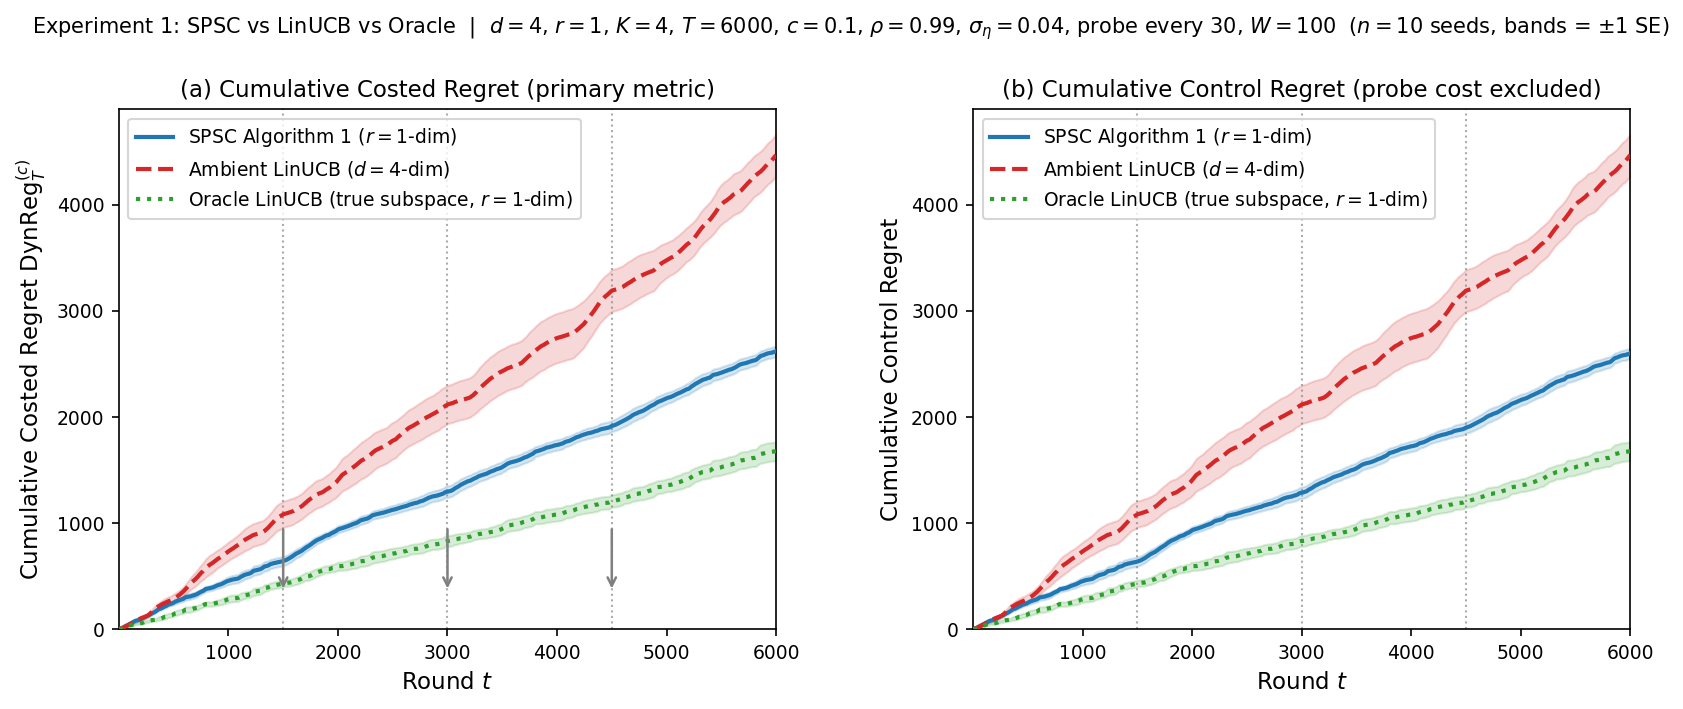
\includegraphics[width=\textwidth]{experiment1_main_benchmark.png}
    \caption{Main synthetic benchmark ($d{=}4$, $r{=}1$, $K{=}4$, $T{=}6000$, 10 seeds).
    Left: cumulative costed regret. Right: cumulative control regret.
    SPSC substantially improves over ambient LinUCB while remaining above the oracle ceiling.}
    \label{fig:main-benchmark}
\end{figure}

\paragraph{Experiment 3: Probe-rate ablation.}
Sweeping probe period over $\{5,10,20,30,50,100,300\}$ reveals a clear U-shaped tradeoff: very sparse probing gives poor subspace estimates, while very frequent probing wastes exploitation rounds.
The optimal performance occurs at intermediate probe frequency ($\sim$20--30), exactly as predicted by the theory.
A direct monotone relationship between late-segment subspace error and final control regret confirms that SPSC's gains are tightly connected to representation quality (Figure~\ref{fig:probe-ablation}).

\begin{figure}[t]
    \centering
    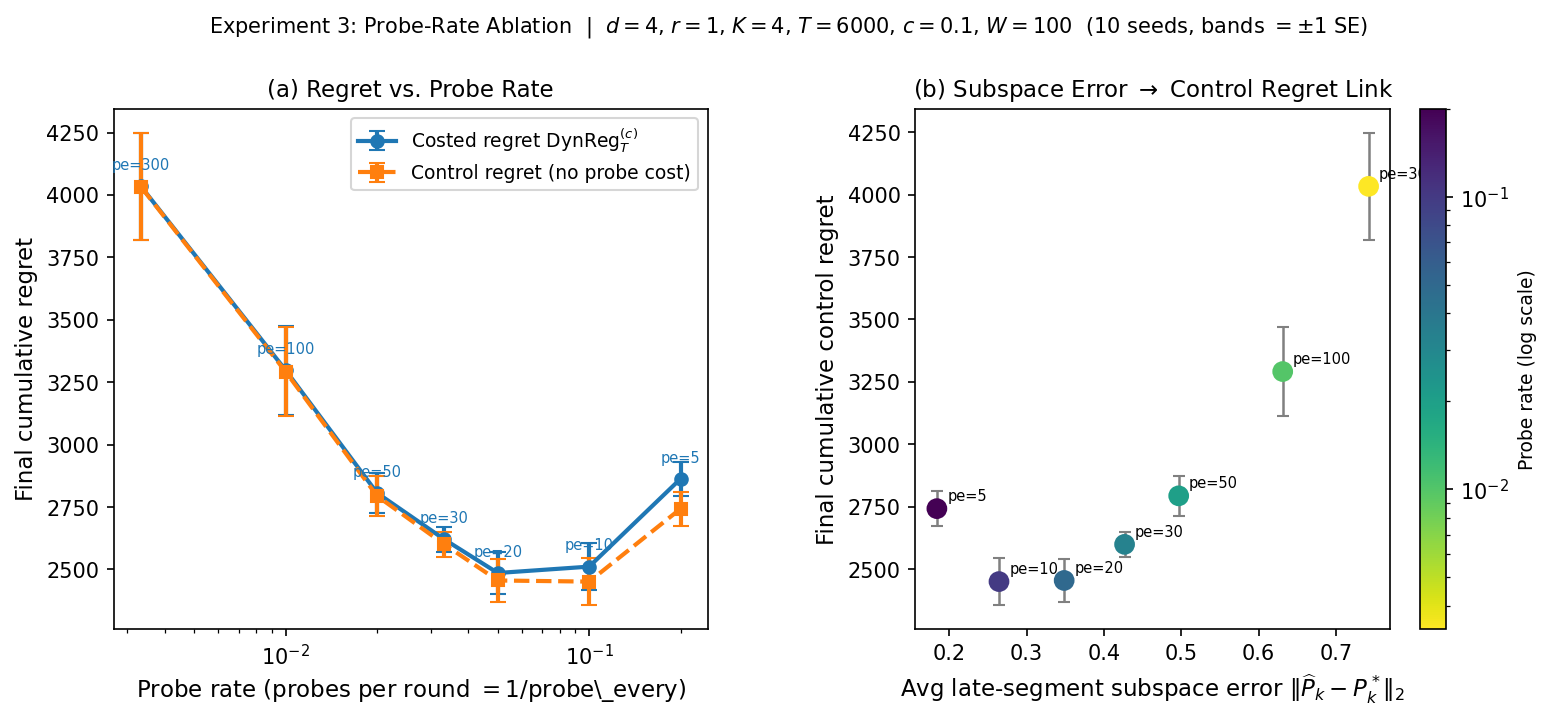
\includegraphics[width=\textwidth]{experiment3_probe_ablation.png}
    \caption{Probe-rate ablation. Left: U-shaped regret vs.\ probe frequency. Right: control regret vs.\ subspace error.}
    \label{fig:probe-ablation}
\end{figure}

\paragraph{Phase diagram on Pendigits.}
We use the UCI Pendigits dataset~\citep{alimoglu1996methods} to construct a semi-synthetic benchmark.
For each $(d,r)$ pair on the grid $d \in \{6,8,10,14,20,30\}$ and $r \in \{1,2,3,5\}$, we run SPSC, LinUCB, and Oracle-LinUCB ($K=4$, $T=5000$, 15 seeds per cell, $24 \times 3 \times 15 = 1080$ runs).
SPSC achieves lower regret than LinUCB in \textbf{23 of 24} grid cells, with improvements ranging from 2\% to 38\%.
The advantage is most pronounced at low $d$ and higher $r$; it fades with $d$ as subspace estimation cost increases; and SPSC never catastrophically underperforms LinUCB (the single loss has ratio 1.05).

\begin{figure}[t]
    \centering
    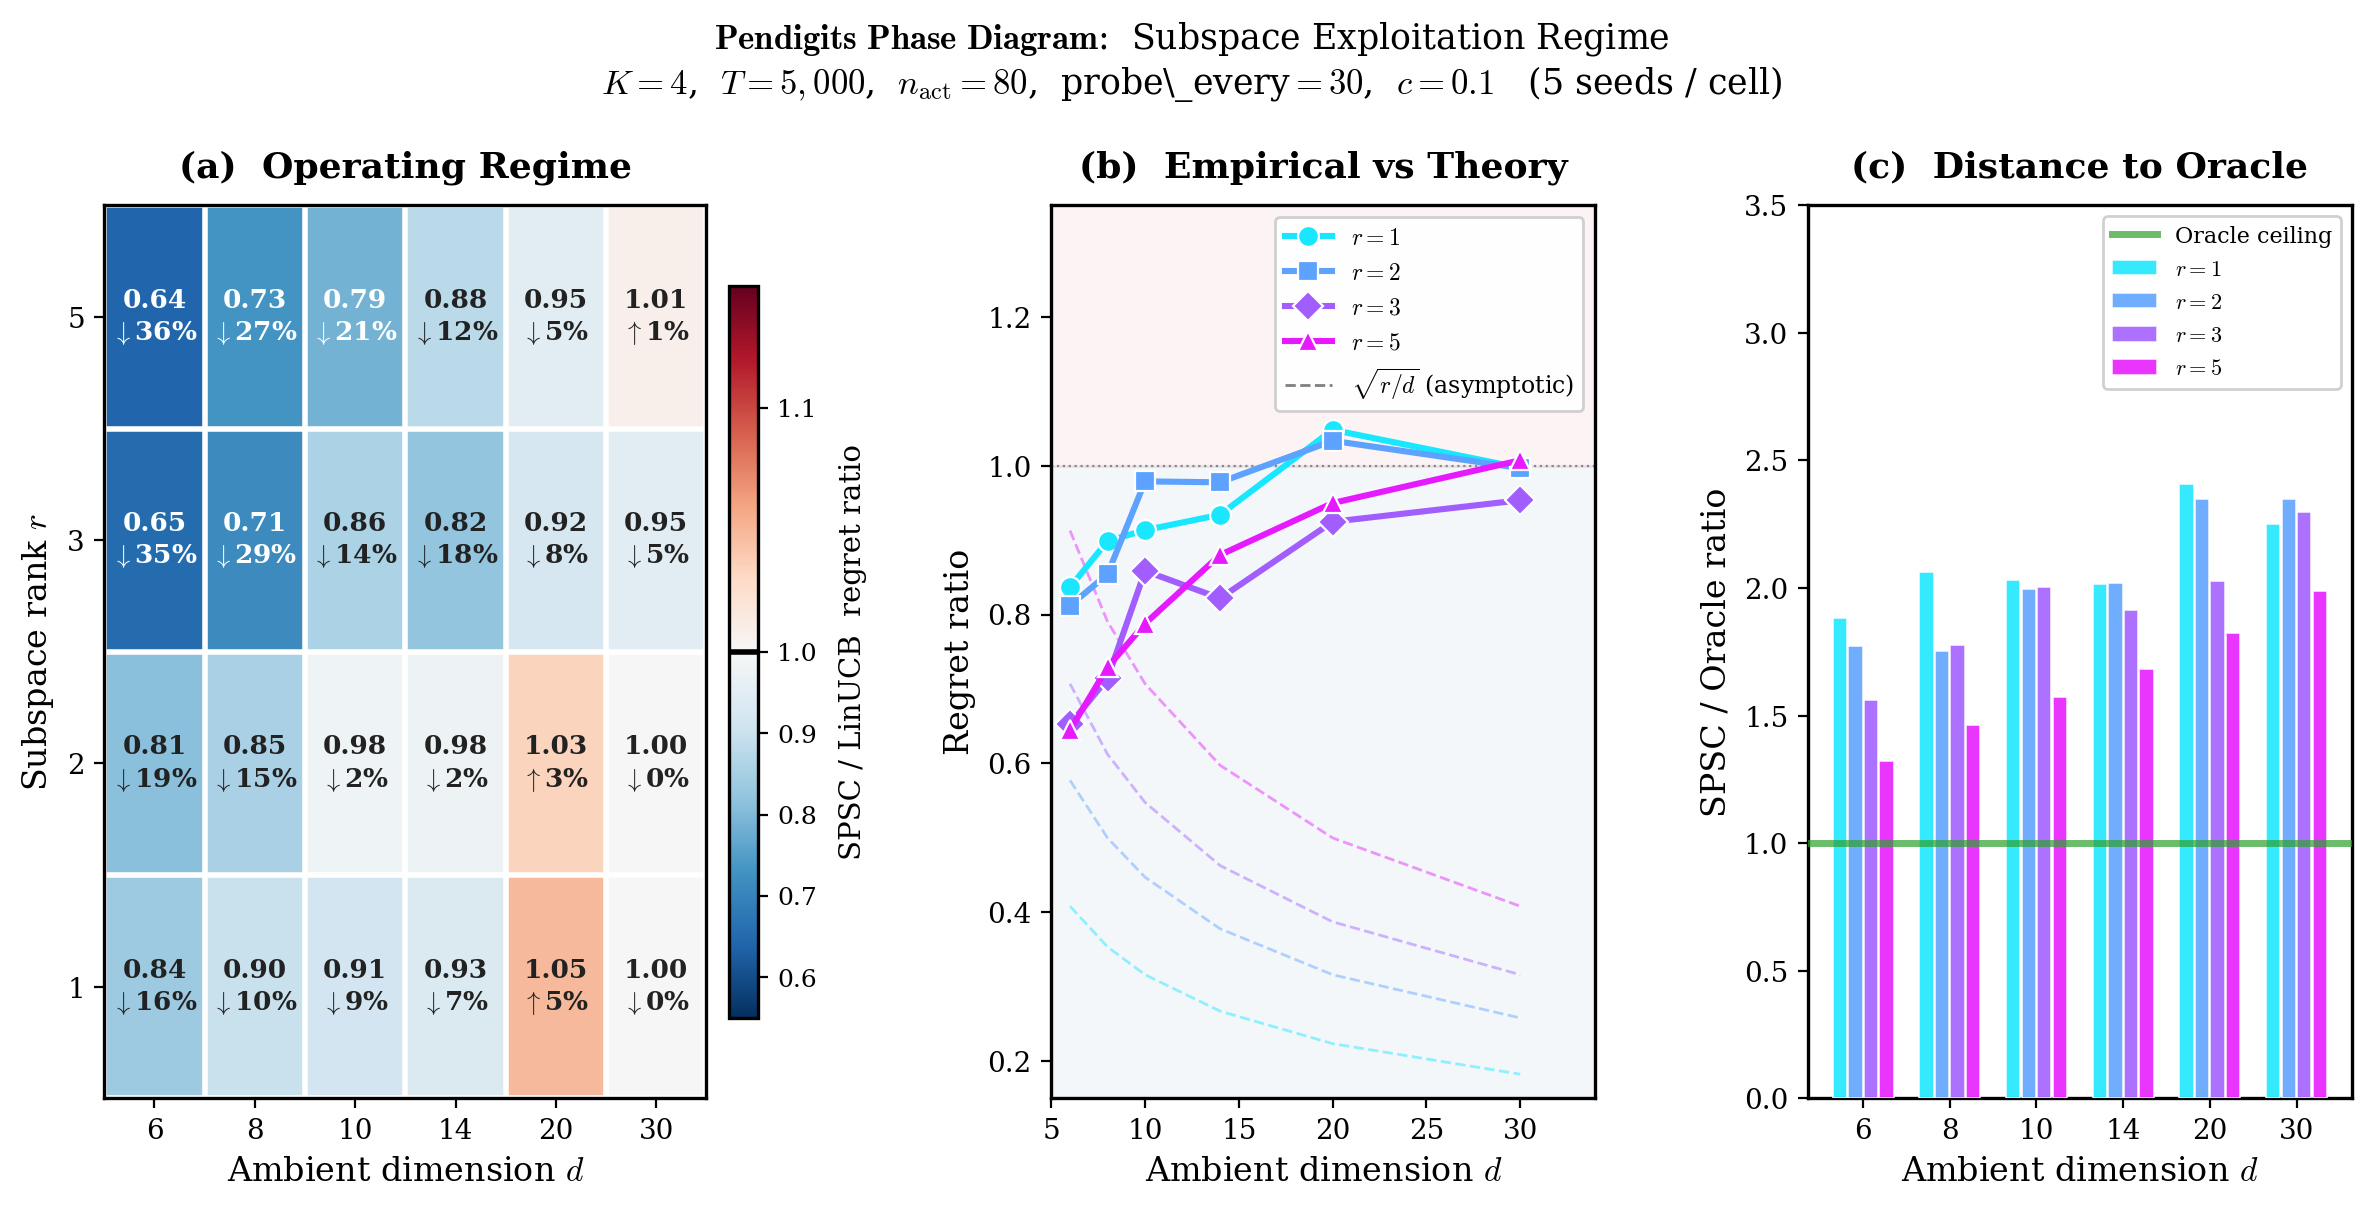
\includegraphics[width=\textwidth]{experiment_phase_diagram.png}
    \caption{Phase diagram on Pendigits ($K{=}4$, $T{=}5000$, 15 seeds per cell).
    (a) SPSC/LinUCB regret ratio heatmap. (b) Empirical ratio vs.\ $\sqrt{r/d}$ prediction. (c) SPSC/Oracle ratio.}
    \label{fig:phase-diagram}
\end{figure}

\paragraph{Satimage 7-method comparison.}
Using the UCI Satimage dataset~\citep{srinivasan1990statlog}, we compare SPSC against six baselines (LinUCB, D-LinUCB~\citep{russac2019weighted}, SW-LinUCB~\citep{cheung2019learning}, Restart-LinUCB~\citep{auer2019adaptively}, LowRank-Reward-UCB~\citep{lu2021low}, and Oracle-LinUCB) across $d \in \{18,24,30,36\}$ and $r \in \{1,2,3,5\}$ (16 cells, 15 seeds, 1680 total runs).
Results are summarized in Table~\ref{tab:satimage_wins}.
SPSC wins all 16 cells against LinUCB, D-LinUCB, and Restart-LinUCB (average reductions of 20--24\%), and 13 of 16 against SW-LinUCB (average ratio 0.94).

\begin{table}[t]
\centering
\small
\begin{tabular}{lcc}
\toprule
Baseline & Cells where SPSC wins & Avg SPSC/Baseline ratio \\
\midrule
LinUCB         & 16/16 & 0.765 \\
D-LinUCB       & 16/16 & 0.797 \\
Restart-LinUCB & 16/16 & 0.774 \\
SW-LinUCB      & 13/16 & 0.936 \\
LowRank-Reward & 9/16  & 0.930 \\
\bottomrule
\end{tabular}
\caption{Satimage benchmark ($d \in \{18,24,30,36\}$, $r \in \{1,2,3,5\}$, $K=4$, $T=5000$, 15 seeds per cell).}
\label{tab:satimage_wins}
\end{table}

\begin{figure}[t]
    \centering
    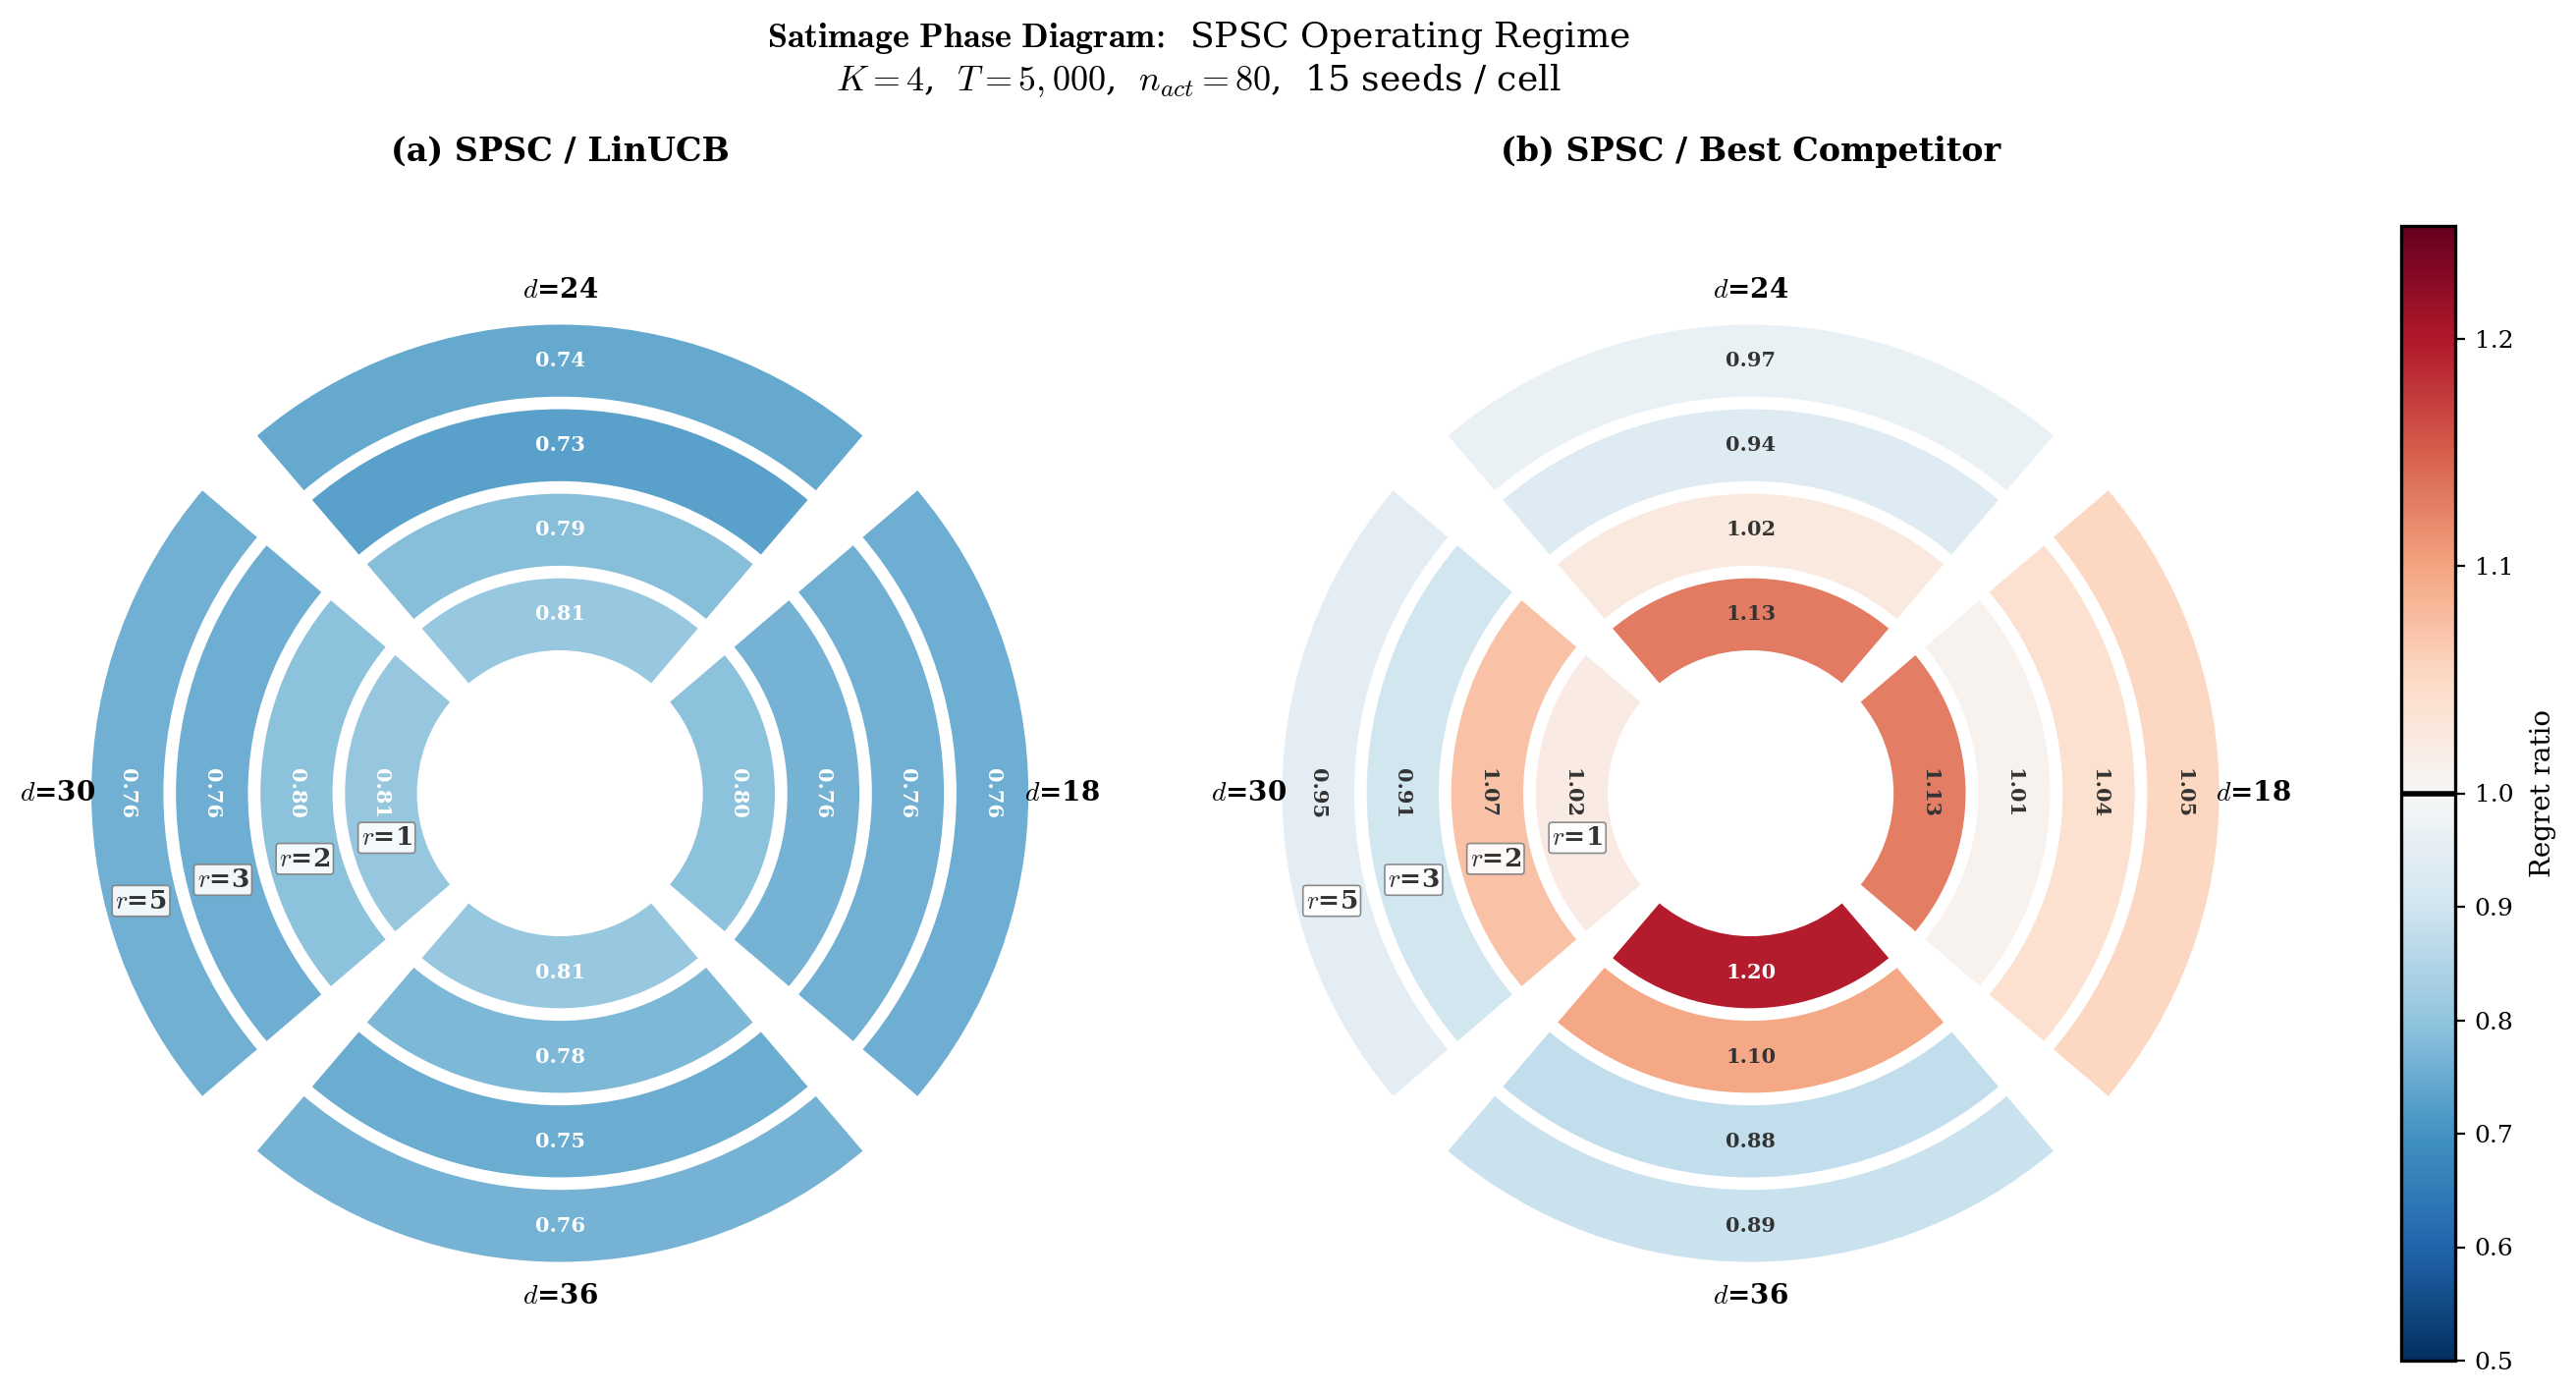
\includegraphics[width=\textwidth]{satimage_double_rings.png}
    \caption{Satimage operating regime. (a) SPSC/LinUCB ratio (entirely blue, 19--27\% reduction). (b) SPSC/Best Competitor ratio.}
    \label{fig:satimage-rings}
\end{figure}

%% ============================================================
%%  DISCUSSION
%% ============================================================
\section{Discussion and Limitations}
\label{sec:discussion}

\paragraph{Noise assumptions.}
The identifiability results rely on known noise variance and state--noise orthogonality (Assumption~\ref{assum:probe_noise}).
Corollary~\ref{cor:regret_misspecified_variance} shows graceful degradation under approximate variance knowledge, but fully relaxing these conditions remains open.

\paragraph{Known rank.}
The algorithm requires the latent rank $r$ as input.
Adaptive rank estimation via eigenvalue thresholding on $\widehat{M}_k$ is a natural extension but introduces additional complexity.

\paragraph{Lower bound gap.}
The $\widetilde{O}(T^{2/3})$ probe--subspace tradeoff is an upper bound.
A matching lower bound would require a Fano-type argument over Grassmannian packings; the $\Omega(c^{1/3}T^{2/3})$ lower bound of \citet{tucker2023costly} for costly-observation bandits is consistent with our rate but not directly applicable.

\paragraph{Dimension scaling.}
The theoretical improvement from $d\sqrt{T}$ to $\sqrt{rT}$ is most impactful when $r \ll d$.
The Pendigits phase diagram confirms broad gains, but the synthetic dimension-scaling study (Appendix~\ref{app:additional_experiments}) does not yet cleanly confirm the asymptotic $\sqrt{r/d}$ narrative at moderate $d$.

%% ============================================================
%%  CONCLUSION
%% ============================================================
\section{Conclusion}
\label{sec:conclusion}

We presented SPSC, an algorithm for online decision-making with piecewise-stationary low-rank rewards.
The key mechanism is a three-stage pipeline: single-play probes yield unbiased quadratic measurements of the predictable second moment; a lifted operator converts these to subspace estimates; and projected optimistic control exploits directly in the learned $r$-dimensional space.
This yields a closed regret bound of $\widetilde{O}(\sqrt{rT}) + \widetilde{O}(T^{2/3}) + O(V)$, replacing the ambient $d\sqrt{T}$ dependence with intrinsic rank $r$.
An adaptive variant achieves the same rate without knowledge of segment boundaries.
Experiments on synthetic and semi-synthetic benchmarks confirm consistent improvements of 6--38\% over non-oracle baselines across a broad $(d,r)$ operating regime.

\paragraph{Broader impact.}
This work is primarily theoretical and methodological.
The framework applies to recommendation systems, dynamic pricing, and adaptive control.

\paragraph{Future work.}
Establishing matching information-theoretic lower bounds for the $T^{2/3}$ rate, relaxing state--noise orthogonality, handling unknown latent rank~$r$, and allowing time-varying transition matrices within segments.

\bibliographystyle{plainnat}
\bibliography{references}

%% ============================================================
%%  APPENDIX
%% ============================================================
\newpage
\appendix

%% ============================================================
%%  APPENDIX A: RELATED WORK TABLE
%% ============================================================
\section{Related Work Comparison Table}
\label{app:related_table}

\begin{table*}[!htpb]
\centering
\small
\setlength{\tabcolsep}{4pt}
\renewcommand{\arraystretch}{1.15}
\begin{tabular}{p{3.2cm} p{1.5cm} p{4.8cm} c c p{4.9cm}}
\toprule
\textbf{Reference} & \textbf{Venue/Year} & \textbf{Regret / Theory} & \textbf{Probing?} & \textbf{CP?} & \textbf{Key difference vs.\ our work} \\
\midrule
\cite{kang2022gestt} & NeurIPS'22 & $\tilde O(\sqrt{(d_1+d_2)MrT})$ & Y & N & Stationary; probing not budgeted. \\
\cite{stojanovic2023spectral} & NeurIPS'23 & Entry-wise / subspace recovery & N/Y & N & Emphasizes estimation; no probe-budget. \\
\cite{pmlr-v235-jedra24a} & ICML'24 & $\tilde O(r^{5/4}(m+n)^{3/4}\sqrt{T})$ & Y & N & Stationary; lacks re-learning. \\
\cite{pmlr-v235-jang24e} & ICML'24 & Arm-set-dependent regret & Y & N & Stationary; no CP detection. \\
\cite{pmlr-v235-lin24o} & ICML'24 & Multi-task regret (shared rank-$r$) & N & N & Multi-task; no within-horizon CPs. \\
\cite{russo2023globalLocal} & AAAI'23 & Fixed-confidence lower bounds & Y & N & Pure exploration; not cumulative regret. \\
\cite{cai2024transfer} & AoS'24 & Minimax regret under covariate shift & N & N & Cross-domain transfer; not piecewise. \\
\cite{park2024latentcontinuity} & IEEE TIT'24 & Estimator matches IT lower limits & N & N & Transfers latent structure; no CP tracking. \\
\cite{abbasi2023dynamic} & JMLR'23 & $\tilde O(\sqrt{KN(S+1)})$ & N & Y & Unstructured K-armed; no low-rank. \\
\cite{komiyama2024adr} & JMLR'24 & ADR-bandit finite-time & N & Y & Unstructured; no low-rank + probing. \\
\cite{sekhari2023aurora} & NeurIPS'23 & $O(\min\{\sqrt{T}, d/\Delta\})$ & Y & N & Preference-query; different feedback. \\
\cite{hou2024pslb} & NeurIPS'24 & Fixed-confidence sample complexity & Y & Y & BAI objective; no low-rank. \\
\cite{pmlr-v267-lazzaro25a} & ICML'25 & Instance-dependent lower bounds & Y & Y & 1D CP localization; not low-rank. \\
\cite{memmel2024asid} & ICLR'24 & Fisher-information exploration & Y & N & Control/system ID; not bandits. \\
\cite{xu2025leqr} & ICLR'25 & $\tilde O(\log N)$ or $\tilde O(\sqrt{N})$ regret & Y & N & Adaptive control; probing via excitation. \\
\bottomrule
\end{tabular}
\caption{Comparison with recent literature. ``CP'' denotes change-point/piecewise stationarity.}
\label{tab:related_work_summary}
\end{table*}

%% ============================================================
%%  APPENDIX B: NOTATION TABLE
%% ============================================================
\section{Notation Table}
\label{app:notation}

\footnotesize
\setlength{\tabcolsep}{4pt}
\renewcommand{\arraystretch}{1.3}

\begin{longtable}{@{}p{0.14\textwidth} p{0.24\textwidth} p{0.08\textwidth} p{0.44\textwidth}@{}}
\toprule
\textbf{Symbol} & \textbf{Meaning} & \textbf{Known?} & \textbf{Assumptions / role} \\
\midrule
\endfirsthead
\toprule
\textbf{Symbol} & \textbf{Meaning} & \textbf{Known?} & \textbf{Assumptions / role} \\
\midrule
\endhead
\bottomrule
\endfoot
$t, T$ & Round index, horizon & Yes & $t=1,\dots,T$. \\
$d, r$ & Ambient \& latent dim. & Yes & $r\ll d$; both assumed known. \\
$K$ & Number of segments & Alg.~1: Yes & Known for Alg.~1; estimated by detector in Alg.~2. \\
$\cA_t$ & Action set at $t$ & Yes & Revealed; bounded by $L_x$. \\
$x_t^{\mathrm{dep}}$ & Deployed action & Yes & Action played; used in regret. \\
$y_t$ & Observed reward & Yes & $y_t=(x_t^{\mathrm{dep}})^\top\theta_t+\varepsilon_t$. \\
$\theta_t$ & Latent reward param. & No & $\theta_t = B_k^\star w_t$. \\
$B_k^\star$ & Representation matrix & No & $d\times r$, orthonormal columns; piecewise constant. \\
$w_t$ & Latent state & No & Evolves via LDS within segment $k$. \\
$A_k$ & LDS transition matrix & No & $\rho(A_k)\le 1-\alpha$. \\
$\widetilde M_t$ & Predictable 2nd-moment & No & $\E[\theta_t\theta_t^\top\mid\cH_{t-1}]$; time-varying. \\
$P_k^\star$ & True seg.\ projector & No & $P_k^\star=B_k^\star(B_k^\star)^\top$. \\
$s_t$ & Centered probe stat. & Derived & $s_t=y_t^2-\sigma_\varepsilon^2$. \\
$G_t$ & Lifted probe sample & Derived & $G_t=\mathcal K^{-1}(s_tu_tu_t^\top)$; unbiased for $\widetilde M_t$. \\
$\widehat M_k$ & Empirical seg.\ estimator & Derived & Unbiased for $\bar M_k^{\mathrm{probe}}$. \\
$\widehat P_k$ & Estimated projector & Derived & Top-$r$ eigenprojector of $\widehat M_k$. \\
$R_X$ & Concentration radius & Derived & $R_X=C_{\mathcal K}L^2R_s+S_w^2$. \\
$C_{\mathrm{sub}}$ & Projector const. & Derived & $C_{\mathrm{sub}}=8R_X/\lambda_{\min}$. \\
$\DynReg_T^{(c)}$ & Costed dynamic regret & No & Performance metric. \\
\end{longtable}
\normalsize

%% ============================================================
%%  APPENDIX C: OMITTED IDENTIFICATION MATERIAL
%% ============================================================
\section{Omitted Identification Material}
\label{app:omitted_identification}

\subsection{Remarks from Problem Setup}

\begin{remark}[Stability margin]
\label{rem:stability_margin}
The algorithm only requires a known lower bound $\alpha_0 \le \alpha$ on the true stability margin.
Any positive $\alpha_0$ certifying strict stability suffices; it can be chosen conservatively small without affecting the regret rates.
\end{remark}

\begin{remark}[Probe design condition]
\label{rem:probe_design}
The condition $\E[uu^\top] \succeq \rho I_d$ requires the probe distribution to have positive second moment in every direction in $\R^d$, ensuring that probe actions span the ambient space.
For isotropic Gaussian probes, $\mathcal{K}^{-1}(N) = \frac{1}{2}N - \frac{\tr(N)}{2(d+2)} I_d$, and $C_{\mathcal K} := \|\mathcal{K}^{-1}\|_{\op} \le 1$.
\end{remark}

\begin{remark}[Noise robustness]
\label{rem:noise_robustness}
When only an estimate $\hat\sigma_\varepsilon^2$ is available with $|\hat\sigma_\varepsilon^2 - \sigma_\varepsilon^2| \le \delta_\sigma$, the regret acquires an extra additive term of order $O(\delta_\sigma T/\lambda_{\min})$ (Corollary~\ref{cor:regret_misspecified_variance}).
Setting $\delta_\sigma = O(T^{-1/3})$ via a burn-in pre-estimation phase keeps this at $\widetilde O(T^{2/3})$.
\end{remark}

\subsection{Biased measurement under variance misspecification}

\begin{proposition}[Biased measurement under variance misspecification]
\label{prop:biased_measurement}
Let $\delta_\sigma := \hat\sigma_\varepsilon^2 - \sigma_\varepsilon^2$ and $\widetilde B := \delta_\sigma\,\mathcal K^{-1}(\Sigma_Q)$.
Then for every probe round $t\in\cTprobe$,
$\E[\hat G_t \mid \cH_{t-1}] = \widetilde M_t - \widetilde B$,
and $\|\widetilde B\|_2 \le |\delta_\sigma|\,C_{\mathcal K}\,L^2$.
The bias is deterministic and rank-$d$; for isotropic Gaussian probes it is a scaled identity $\widetilde B \approx \frac{\delta_\sigma}{2}I_d$, so eigenvectors of $\bar M_k^{\mathrm{probe}}$ are not corrupted---only eigenvalues are shifted.
\end{proposition}

\subsection{Non-identification results}

\paragraph{Impossibility: all three conditions are necessary.}
Three complementary results show that dropping any single condition destroys identifiability:

\begin{proposition}[Non-identification]
  \label{prop:nonid}
  \leavevmode
  \begin{enumerate}[label=(\alph*), itemsep=1pt]
    \item \textbf{Without known noise variance} (Proposition~6 in the full version): for any $\widetilde{M}_t$, there exists $\widetilde{M}_t' \neq \widetilde{M}_t$ and a noise variance function $v'_t(u)$ that produce identical observations.
    \item \textbf{Without state--noise orthogonality} (Proposition~7): for any nonzero symmetric $H$, there exist modified cross-moments that replicate all observable quadratics.
    \item \textbf{Without full-dimensional coverage} (Proposition~8): if all probe actions lie in a proper subspace $S \subsetneq \R^d$, no signal outside $S$ is detectable from either linear or quadratic observations.
  \end{enumerate}
\end{proposition}

\begin{remark}[Joint necessity]
\label{rem:joint_necessity}
No two of the three conditions are jointly sufficient; all three are simultaneously required.
Proposition~\ref{prop:nonid}(a) shows failure even with (iii) and full coverage when (ii) is dropped.
Proposition~\ref{prop:nonid}(b) shows failure even with (ii) and full coverage when (iii) is dropped.
Proposition~\ref{prop:nonid}(c) shows failure even with (ii) and (iii) when coverage is restricted.
\end{remark}

\paragraph{Structural justification: the role of probing.}
In a static setting, passive methods can eventually learn the subspace from exploitation data alone.
However, in our piecewise non-stationary setting, the subspace changes at each change point, invalidating all previously learned structure.
Deployed actions chosen for exploitation tend to align with the learner's current (now outdated) estimate, collapsing into a restricted proper subspace $S \subset \R^d$.
Proposition~\ref{prop:nonid}(c) shows that measurements confined to $S$ cannot identify the new subspace.
Assumption~\ref{assum:probe_realizability} resolves this by guaranteeing full-dimensional probe coverage.
The quantitative necessity of full-dimensional coverage is formalized in Appendix~\ref{app:coverage_lower_bound}, where Theorem~\ref{thm:restricted_span_minimax_regret} shows that restricting deployed actions to any proper subspace forces $\Omega(T)$ regret.

%% ============================================================
%%  APPENDIX D: SUPPORTING REGRET THEOREMS
%% ============================================================
\section{Supporting Regret Theorems}
\label{app:supporting_regret}

\begin{theorem}[Segmentwise windowed exploitation regret]
\label{thm:segment_windowed_projected}
Fix a segment $\cI_k$. Under standard conditions (orthonormal $B_k^\star$, bounded $\|w_t\|_2 \le S_w$, bounded actions, subspace error $\varepsilon_k$, conditionally sub-Gaussian noise on exploitation rounds), with probability at least $1-\delta$, the exploitation regret in segment $k$ satisfies
\[
R_k^{\mathrm{exp}} \le
2\beta_k^{(r,W)}
\sqrt{2r n_k \log\!\left(1+\frac{W L_x^2}{\lambda r}\right)}
+ 2S_wL_x \varepsilon_k n_k
+ 2L_x \sum_{t\in E_k} V_{k,t}(W),
\]
where $n_k:=|E_k|$.
\end{theorem}

\begin{theorem}[Full-horizon windowed dynamic regret]
\label{thm:full_horizon_windowed}
Under the hypotheses of Theorem~\ref{thm:segment_windowed_projected} on every segment, with probability at least $1-\delta$,
\[
\DynReg_T^{(c)} \le
(2L_xS_w+c)\sum_{k=1}^K m_k
+ 2\sum_{k=1}^K \beta_k^{(r,W)}
\sqrt{2r n_k \log\!\left(1+\frac{W L_x^2}{\lambda r}\right)}
+ 2S_wL_x \sum_{k=1}^K \varepsilon_k n_k
+ 2L_xW \sum_{k=1}^K V_k.
\]
\end{theorem}

\paragraph{Concentration results.}
The centered lifted samples $X_t := G_t - \widetilde{M}_t$ form a bounded matrix martingale difference sequence with $\|X_t\|_2 \le R_X$.
The Matrix Freedman inequality~\citep{tropp2012user} yields:

\begin{theorem}[Empirical matrix concentration]
\label{thm:matrix_concentration_summary}
With probability at least $1-\delta$:
$\|\widehat{M}_k - \bar{M}_k^{\mathrm{probe}}\|_2 \le 2R_X \sqrt{\log(2d/\delta)/m_k}$.
\end{theorem}

\begin{theorem}[Projector concentration]
\label{thm:projector_concentration_summary}
If $m_k$ is large enough that $\|\widehat M_k - \bar M_k^{\mathrm{probe}}\|_2 \le \lambda_{\min}/2$, then with probability at least $1-\delta$:
$\|\widehat{P}_k - P_k^\star\|_2 \le C_{\mathrm{sub}}\sqrt{\log(2d/\delta)/m_k}$, where $C_{\mathrm{sub}} := 8R_X/\lambda_{\min}$.
\end{theorem}

\begin{remark}[Rate interpretation and parameter tuning]
\label{rem:adaptive_rate_discussion}
\textbf{On $\hat K$ vs.\ $K$.}  The random variable $\hat K$ denotes the total number of resets triggered by the detector.  On the high-probability event ($\Prob \ge 1-\delta$) that $F_T = 0$, we have $\hat K = K$ exactly, so the oracle-equivalent term in \eqref{eq:adaptive_regret_bound} recovers the rate of Theorem~\ref{thm:closed_dynamic_regret} with $K$ in place of $\hat K$.  The detection-delay penalty scales as $K D_{\max} = K((2n/\mu) + \tau_{\mathrm{burn}})$ and the recovery cost scales as $K m_{\mathrm{relearn}}$.  For fixed $K$, these are $O(1)$ in $T$ and therefore absorbed into the lower-order $AK$ term, provided $n$ and $m_{\mathrm{relearn}}$ are constants independent of $T$.  The minimum detectable change magnitude is $\Delta_{\mathrm{det}} = 2b = O(R_X\sqrt{\log(dT)/n})$, which decreases as $n$ increases.  When $K$ is unknown but $K = O(T^\beta)$ for some $\beta \in [0, 1)$, the overhead terms are polynomial in $T$ but dominated by the $T^{2/3}$ term as long as $K = o(T^{2/3})$.
\end{remark}

\begin{remark}[Absence of a matching lower bound]
\label{rem:lower_bound}
The $\widetilde O(T^{2/3})$ rate is an upper bound only.
A matching lower bound would require a Fano-type argument constructing $\exp(\Omega(r\log d))$ subspaces; this is left for future work.
The $\Omega(c^{1/3}T^{2/3})$ lower bound of \citet{tucker2023costly} for costly-observation bandits is consistent with this rate.
\end{remark}

%% ============================================================
%%  APPENDIX E: CONCENTRATION PROOFS
%% ============================================================
\section{Concentration Inequalities for Subspace Recovery}
\label{app:concentration}

During segment $k$, the learner computes $\widehat{M}_k = \frac{1}{m_k} \sum_{t \in \cT_k} G_t$.
From Proposition~\ref{prop:lifted_probe_unbiased}, $X_t := G_t - \widetilde{M}_t$ is a martingale difference sequence with $\E[X_t \mid \cH_{t-1}] = 0$.
Throughout, Assumptions~\ref{assum:latent_dynamics}--\ref{assum:bounded_probe_noise} hold and $\|w_t\|_2 \le S_w$.

\begin{lemma}[Uniform bound on probe statistic]
\label{lem:st_uniform_bound}
On every probe round, $|s_t| \le R_s := (LS_w + L_\varepsilon)^2 + \sigma_\varepsilon^2$.
\end{lemma}

\begin{proof}
$|y_t| \le LS_w + L_\varepsilon$ and $|s_t| \le |y_t|^2 + \sigma_\varepsilon^2 \le R_s$.
\end{proof}

\begin{lemma}[Lifted probe MDS]
\label{lem:lifted_mds}
$\E[X_t \mid \cH_{t-1}] = 0$ and $\widehat{M}_k - \bar{M}_k^{\mathrm{probe}} = \frac{1}{m_k}\sum_{t \in \cT_k} X_t$.
\end{lemma}

\begin{lemma}[Uniform operator norm bound]
\label{lem:uniform_operator_bound}
$\|X_t\|_2 \le R_X := C_{\mathcal K}\,L^2\,R_s + S_w^2$.
\end{lemma}

\begin{proof}
$\|G_t\|_2 \le C_{\mathcal K} R_s L^2$ and $\|\widetilde{M}_t\|_2 \le S_w^2$, so $\|X_t\|_2 \le C_{\mathcal K} L^2 R_s + S_w^2$.
\end{proof}

\begin{lemma}[Predictable quadratic variation]
\label{lem:variance_bound}
$\|\sum_{t \in \cT_k} \E[X_t^2 \mid \cH_{t-1}]\|_2 \le m_k R_X^2$.
\end{lemma}

\begin{theorem}[Segment-level concentration]
\label{thm:matrix_concentration_app}
For every segment $k$ and $\delta \in (0,1)$, with probability at least $1-\delta$:
$\|\widehat{M}_k - \bar{M}_k^{\mathrm{probe}}\|_2 \le 2R_X \sqrt{\log(2d/\delta)/m_k}$.
\end{theorem}

\begin{proof}
The partial sums $Y_j = \sum_{t \in \cT_k,\, t \le j} X_t$ form a self-adjoint matrix martingale with $\|X_t\|_2 \le R_X$ and variance proxy $m_k R_X^2$.
The Matrix Freedman inequality~\citep{tropp2012user} with $u = 2R_X\sqrt{m_k\log(2d/\delta)}$ gives
$\Prob(\|\sum X_t\|_2 \ge u) \le 2d\exp(-u^2/2/(m_k R_X^2 + R_X u/3)) \le \delta$.
Dividing by $m_k$ yields the result.
\end{proof}

\begin{theorem}[Biased concentration under variance misspecification]
\label{thm:biased_concentration}
Let $\hat R_X := R_X + 2C_{\mathcal K}|\delta_\sigma|L^2$.
With probability at least $1-\delta$:
$\|\widehat M_k^{\hat\sigma} - (\bar M_k^{\mathrm{probe}} - \widetilde B)\|_2 \le 2\hat R_X\sqrt{\log(2d/\delta)/m_k}$.
Consequently, $\|\widehat M_k^{\hat\sigma} - \bar M_k^{\mathrm{probe}}\|_2 \le 2\hat R_X\sqrt{\log(2d/\delta)/m_k} + C_{\mathcal K}|\delta_\sigma|L^2$.
\end{theorem}

\begin{proof}
The centered residuals $\hat X_t := \hat G_t - \E[\hat G_t \mid \cH_{t-1}]$ form a MDS with $\|\hat X_t\|_2 \le \hat R_X$.
The Matrix Freedman inequality yields the first bound; the triangle inequality with $\|\widetilde B\|_2 \le C_{\mathcal K}|\delta_\sigma|L^2$ gives the second.
\end{proof}

\subsection{Davis--Kahan and projector recovery}

\begin{theorem}[Segment projector recovery]
\label{thm:davis_kahan_application}
If $\|\widehat{M}_k - \bar{M}_k^{\mathrm{probe}}\|_2 \le \lambda_{\min}/2$, then with probability at least $1-\delta$:
$\|\widehat{P}_k - P_k^\star\|_2 \le \frac{8R_X}{\lambda_{\min}} \sqrt{\log(2d/\delta)/m_k}$.
\end{theorem}

\begin{proof}
By Weyl's inequality, $\lambda_r(\widehat{M}_k) \ge \lambda_{\min}/2$ and $\lambda_{r+1}(\widehat{M}_k) \le \lambda_{\min}/2$.
The $\sin\Theta$ perturbation bound~\citep{davis1970rotation,yu2015useful} gives $\|\widehat{P}_k - P_k^\star\|_2 \le 4\|E\|_2/\lambda_{\min}$.
Substituting $\|E\|_2 \le 2R_X\sqrt{\log(2d/\delta)/m_k}$ from Theorem~\ref{thm:matrix_concentration_app} yields the result.
\end{proof}

\begin{corollary}[Projector recovery under misspecification]
\label{cor:projector_misspec}
If $C_{\mathcal K}|\delta_\sigma|L^2 \le \lambda_{\min}/4$ and $m_k \ge 64\hat R_X^2\log(2d/\delta)/\lambda_{\min}^2$, then
$\|\widehat P_k - P_k^\star\|_2 \le \hat C_{\mathrm{sub}}\sqrt{\log(2d/\delta)/m_k} + \Delta_\sigma$,
where $\hat C_{\mathrm{sub}} := 8\hat R_X/\lambda_{\min}$ and $\Delta_\sigma := 4C_{\mathcal K}|\delta_\sigma|L^2/\lambda_{\min}$.
\end{corollary}

\subsection{Detector guarantees}

\begin{lemma}[Within-segment second-moment variation]
\label{lem:within_segment_variation}
Under Assumption~\ref{assum:latent_dynamics}, for $s < t$ in the same segment with both at least $\tau_{\mathrm{burn}}$ rounds after the segment start,
$\|\widetilde M_t - \widetilde M_s\|_{\op} \le \Delta_{\mathrm{within}}(\tau_{\mathrm{burn}}) := 2(1-\alpha_0)^{2\tau_{\mathrm{burn}}} S_w^2/(1-(1-\alpha_0)^2)$.
\end{lemma}

\begin{theorem}[No-change control]
\label{thm:no_change_control}
If no change point falls within the combined detector window and both windows begin at least $\tau_{\mathrm{burn}}$ rounds after the most recent change point, then for any fixed $t$:
$\Prob(S_t > b) \le \delta_{\mathrm{FA}}/T$,
and the total number of false alarms satisfies $\E[F_T] \le \delta_{\mathrm{FA}}$, so $F_T = 0$ with probability at least $1 - \delta_{\mathrm{FA}}$.
\end{theorem}

\begin{proof}
Under no change, both window estimates have within-segment targets satisfying $\|\bar M^{\mathrm{recent}} - \bar M^{\mathrm{past}}\|_{\op} \le \Delta_{\mathrm{within}}$ by Lemma~\ref{lem:within_segment_variation}.
By Theorem~\ref{thm:matrix_concentration_app} applied independently to each window at confidence $\delta_{\mathrm{FA}}/(2T)$, the triangle inequality and union bound give $S_t \le b$ with probability $\ge 1 - \delta_{\mathrm{FA}}/T$.
\end{proof}

\begin{theorem}[Post-change detection]
\label{thm:post_change_detection}
If $\Delta_k \ge \Delta_{\mathrm{det}} = 2b$, then with probability at least $1 - \delta/(K+1)$, the detector fires within delay $D_k \le D_{\max} := (n_r + n_p)/\mu + \tau_{\mathrm{burn}}$.
\end{theorem}

\begin{proof}
At the first round $t^\star \le \tau_k + D_{\max}$ where the recent window lies entirely post-change and the past window entirely pre-change, the reverse triangle inequality gives $S_{t^\star} \ge \Delta_k - b > b$, so the detector fires.
\end{proof}

%% ============================================================
%%  APPENDIX F: MATHEMATICAL SEPARATIONS
%% ============================================================
\section{Mathematical Separations from Prior Work}
\label{app:separation}

\begin{proposition}[Our model is not reducible to Qin's task-constant model]
\label{prop:separation_qin_1}
Fix $N\ge 2$. There exist instances of our model for which $\Prob(\theta_t = \theta_{t+1}) = 0$ for all $t$ within any segment.
\end{proposition}

\begin{proof}
Take $B_k^\star = [I_r; 0]$, $A_k = 0$, $\eta_t \stackrel{\mathrm{i.i.d.}}{\sim} \mathcal N(0,I_r)$.
Then $w_t = \eta_{t-1}$ are i.i.d.\ Gaussian, so $\Prob(\theta_t = \theta_{t+1}) = 0$.
\end{proof}

\begin{proposition}[Identifiable instance not covered by Qin's mechanism]
\label{prop:separation_qin_2}
With $r\ge 2$, one segment, $A_k = 0$, $\Sigma_{\eta,k} = I_r$: our Proposition~\ref{prop:subspace_identification} gives $\range(\bar M_k^{\mathrm{probe}})=\range(B_k^\star)$.
But with $N=1$ task, Qin's task-covariance has rank $\le 1 < r$.
\end{proposition}

\begin{proposition}[Finite probe actions do not identify a changing ambient subspace]
\label{prop:separation_elu_1}
If probe directions lie in a finite set $U \subset \R^d$ with $\Span(U) \neq \R^d$, then $\widetilde M_t$ is not identifiable from $\{u_i^\top \widetilde M_t u_i : u_i \in U\}$.
\end{proposition}

%% ============================================================
%%  APPENDIX G: AMBIENT REFERENCE BOUND
%% ============================================================
\section{Ambient-Space Reference Bound}
\label{app:ambient_reference}

\begin{theorem}[Ambient-space costed dynamic regret]
\label{thm:ambient_regret}
Under Assumptions~\ref{assum:latent_dynamics}--\ref{assum:bounded_probe_noise}, with probability at least $1-\delta$:
\[
    \DynReg_T^{(c)} \le \underbrace{(2 L_x S_w + c) m_T}_{\text{probing cost}}
    + \underbrace{\tilO(d \sqrt{T})}_{\text{ambient statistical regret}}
    + \underbrace{\tilO\!\left( \frac{S_w L_x R_X}{\lambda_{\min}} \sum_{t \notin \cTprobe} \frac{1}{\sqrt{m_{t-1}}} \right)}_{\text{subspace approximation error}}.
\]
Under a uniform probe schedule, this yields $\tilO(d\sqrt{T} + T^{2/3})$, compared to $\tilO(\sqrt{rT} + T^{2/3})$ from Theorem~\ref{thm:closed_dynamic_regret}.
The improvement from $d\sqrt{T}$ to $\sqrt{rT}$ is achieved by the projected exploitation layer.
\end{theorem}

%% ============================================================
%%  APPENDIX H: PROJECTED EXPLOITATION ANALYSIS
%% ============================================================
\section{Projected Exploitation in the Learned Subspace}
\label{app:projected_exploitation}

\subsection{Supporting lemmas}

\begin{lemma}[Self-normalized inequality in dimension $r$]
\label{lem:self_normalized_r}
Let $M_t := \sum_{s=1}^t z_s \eta_s$, $V_t := \lambda I_r + \sum_{s=1}^t z_s z_s^\top$, where $\eta_s$ is conditionally $\sigma_\varepsilon$-sub-Gaussian. Then for any $\delta\in(0,1)$, with probability at least $1-\delta$, simultaneously for all $t\ge 1$,
$\|M_t\|_{V_t^{-1}} \le \sigma_\varepsilon \sqrt{2\log(\det(V_t)^{1/2}/(\det(\lambda I_r)^{1/2}\delta))}$.
\end{lemma}

\begin{lemma}[Determinant bound]
\label{lem:det_bound_r}
If $\|z_s\|_2\le L_x$, then $\log(\det(V)/\lambda^r) \le r\log(1+N L_x^2/(\lambda r))$.
\end{lemma}

\begin{lemma}[Elliptical potential bound]
\label{lem:elliptical_r}
$\sum_{t=1}^N \|z_t\|_{V_{t-1}^{-1}} \le \sqrt{2rN\log(1+N L_x^2/(\lambda r))}$.
\end{lemma}

\subsection{Segmentwise projected exploitation algorithms}

\begin{algorithm}[t]
\caption{Segmentwise projected ridge-UCB in the learned subspace}
\label{alg:segment_projected_ofu}
\begin{algorithmic}[1]
\State \textbf{Input:} segment $\cI_k$, estimated basis $\widehat U_k$, $\lambda>0$, $\Gamma_k$, $\delta$
\For{each exploitation round $t\in E_k$}
    \State $z_t(x)=\widehat U_k^\top x$ for each $x \in \cA_t$
    \State $\widetilde V_{t-1} = \lambda I_r + \sum_{s<t} z_s z_s^\top$, \; $\widetilde b_{t-1} = \sum_{s<t} z_s y_s$
    \State $\widehat a_t = \widetilde V_{t-1}^{-1}\widetilde b_{t-1}$
    \State $x_t \in \argmax_{x\in \cA_t}\{z_t(x)^\top \widehat a_t + \beta_t^{(r)}\|z_t(x)\|_{\widetilde V_{t-1}^{-1}} + \Gamma_k\|x\|_2\}$
\EndFor
\end{algorithmic}
\end{algorithm}

\begin{algorithm}[t]
\caption{Windowed projected ridge-UCB in the learned subspace}
\label{alg:windowed_projected_ofu}
\begin{algorithmic}[1]
\State \textbf{Input:} segment $\cI_k$, estimated basis $\widehat U_k$, $\lambda>0$, window $W$, $\Gamma_k$, $\delta$
\For{each exploitation round $t\in E_k$}
    \State $\mathcal W_t = \{s\in E_k : t-W \le s < t\}$
    \State $z_t(x)=\widehat U_k^\top x$ for each $x \in \cA_t$
    \State $\widetilde V_t = \lambda I_r + \sum_{s\in \mathcal W_t} z_s z_s^\top$, \; $\widetilde b_t = \sum_{s\in \mathcal W_t} z_s y_s$
    \State $\widehat a_t = \widetilde V_t^{-1}\widetilde b_t$
    \State $x_t \in \argmax_{x\in \cA_t}\{z_t(x)^\top \widehat a_t + \beta_t^{(r,W)}\|z_t(x)\|_{\widetilde V_t^{-1}} + \Gamma_k\|x\|_2 + L_xV_{k,t}(W)\}$
\EndFor
\end{algorithmic}
\end{algorithm}

\begin{theorem}[Segmentwise projected regret under varying $w_t$]
\label{thm:segment_projected_varying}
With probability at least $1-\delta$,
$R_k^{\mathrm{exp}} \le 2\beta_{k,\max}^{(r)} \sqrt{2rn_k\log(1+n_kL_x^2/(\lambda r))} + 2S_wL_x\varepsilon_k n_k + 2L_x \sum_{t\in E_k} D_{k,t}$,
where $D_{k,t} := \|\theta_t - \theta_{\tau_{k-1}}\|_2$.
\end{theorem}

\begin{theorem}[Windowed projected regret under varying $w_t$]
\label{thm:windowed_projected_varying}
With probability at least $1-\delta$, the exploitation regret satisfies
$R_k^{\mathrm{exp}} \le 2\beta_k^{(r,W)} \sqrt{2rn_k\log(1+WL_x^2/(\lambda r))} + 2S_wL_x\varepsilon_k n_k + 2L_x W V_k$.
\end{theorem}

\begin{proof}
Fix $t\in E_k$ and define $a_t^\star := \widehat U_k^\top \theta_t$.
Then $x^\top \theta_t = z_t(x)^\top a_t^\star + x^\top(I-\widehat P_k)\theta_t$, with $|x^\top(I-\widehat P_k)\theta_t| \le \Gamma_k\|x\|_2$.
For past rounds $s\in\mathcal W_t$, the drift error satisfies $|e_{s,t}^{\mathrm{drift}}| \le L_xV_{k,t}(W)$.
The estimation error is bounded by $\beta_t^{(r,W)}\|z\|_{\widetilde V_t^{-1}}$ via Lemmas~\ref{lem:self_normalized_r}--\ref{lem:det_bound_r}.
Summing over $t\in E_k$ and applying Lemma~\ref{lem:elliptical_r} with $\sum_{t\in E_k} V_{k,t}(W) \le W V_k$ yields the result.
\end{proof}

\subsection{Adaptive-reset algorithm pseudocode}
\label{app:adaptive_pseudocode}

\begin{algorithm}[t]
  \caption{Adaptive Single-Play Subspace-Aware Control (Unknown Segment Boundaries)}
  \label{alg:adaptive_reset_control_main}
  \begin{algorithmic}[1]
  \State \textbf{Input:} Probe rate $\mu\in(0,1)$, detection window $n$ ($n_r=n_p=n$),
         threshold $b$ from \eqref{eq:detector_threshold_main},
         burn-in $\tau_{\mathrm{burn}}$, recovery length $m_{\mathrm{relearn}}$,
         $\lambda>0$, $\sigma_\varepsilon^2$, $Q$, $r$, $W$.
  \State \textbf{Initialize:} $\widehat U_0\in\R^{d\times r}$;
         $\widehat P\leftarrow\widehat U_0\widehat U_0^\top$;
         $\widehat M_{\mathrm{acc}}\leftarrow\mathbf{0}$;
         $\mathtt{phase}\leftarrow\textsc{recovery}$;
         $\mathtt{rec\_count}\leftarrow 0$; $n_{\mathrm{pr}}\leftarrow 0$
  \For{$t = 1, \dots, T$}
      \State Observe $\cA_t$.
      \If{$\mathtt{phase} = \textsc{recovery}$}
          \State Draw $u_t\sim Q$; deploy $x_t^{\mathrm{dep}}=u_t$; observe $y_t$.
          \State $s_t = y_t^2-\sigma_\varepsilon^2$; $G_t = \mathcal{K}^{-1}(s_t u_t u_t^\top)$.
          \State $\widehat M_{\mathrm{acc}}\leftarrow \widehat M_{\mathrm{acc}}+G_t$; $\mathtt{rec\_count}\leftarrow\mathtt{rec\_count}+1$.
          \If{$\mathtt{rec\_count}=m_{\mathrm{relearn}}$}
              \State $\widehat U\leftarrow\TopEig_r(\widehat M_{\mathrm{acc}}/m_{\mathrm{relearn}})$;
                     $\widehat P\leftarrow\widehat U\widehat U^\top$.
              \State $n_{\mathrm{pr}}\leftarrow m_{\mathrm{relearn}}$;
                     $\mathtt{rec\_count}\leftarrow 0$;
                     $\mathtt{phase}\leftarrow\textsc{normal}$.
          \EndIf
      \Else
          \If{probe round (determined by probe rate $\mu$)}
              \State Draw $u_t\sim Q$; deploy; compute $G_t$; update $\widehat M_{\mathrm{acc}}$, $\widehat U$, $\widehat P$.
              \If{detection window active and $S_t > b$}
                  \State $\mathtt{phase}\leftarrow\textsc{recovery}$; reset all buffers.
              \EndIf
          \Else
              \State Exploitation: windowed reduced ridge-UCB as in Algorithm~\ref{alg:single_play_control_rdim}.
          \EndIf
      \EndIf
  \EndFor
  \end{algorithmic}
\end{algorithm}

%% ============================================================
%%  APPENDIX I: COVERAGE LOWER BOUNDS
%% ============================================================
\section{Lower Bounds: Necessity of Full Coverage}
\label{app:coverage_lower_bound}

\begin{theorem}[Minimax lower bound under restricted deployed-action span]
\label{thm:restricted_span_minimax_regret}
Let $S \subsetneq \R^d$ be a proper subspace, and let $\Pi(S)$ be the class of all policies with $x_t^{\mathrm{dep}} \in S$ a.s.
Then there exists a subclass $\mathfrak M(S)$ satisfying all structural assumptions such that
$\inf_{\pi \in \Pi(S)} \sup_{\nu \in \mathfrak M(S)} \E_\nu^\pi[\DynReg_T^{(c)}] \ge \mu T$
for some constant $\mu > 0$.
\end{theorem}

\begin{proof}
Fix $v \in S^\perp$, $\|v\|=1$.
Construct a one-segment model with $B_1^\star = v$, $A_1 = 0$, $\eta_t = \mu \xi_t$ (Rademacher), $\cA_t = \{0, v, -v\}$.
Since $v \notin S$, any policy in $\Pi(S)$ must play $x_t^{\mathrm{dep}} = 0$ a.s., while $\max_{x \in \cA_t} x^\top \theta_t = \mu$ a.s.
Hence $\DynReg_T^{(c)} \ge \mu T$ a.s.
\end{proof}

\begin{theorem}[Lower bound when both deployed and probe actions are confined]
\label{thm:restricted_span_minimax_regret_with_probe}
Under the same construction, $\inf_{\pi \in \Pi_{\mathrm{probe}}(S)} \sup_{\nu \in \mathfrak M(S)} \E_\nu^\pi[\DynReg_T^{(c)}] \ge \mu T$.
The probe count is $\nu$-independent (all observations equal $\varepsilon_t$ since $(x_t^{\mathrm{dep}})^\top \theta_t = 0$), so probing within $S$ provides no information about $\theta_t \in S^\perp$.
\end{theorem}

\begin{corollary}[Sublinear regret is impossible without full coverage]
\label{cor:restricted_span_minimax_sublinear_impossible}
No policy in $\Pi(S)$ or $\Pi_{\mathrm{probe}}(S)$ can guarantee $o(T)$ expected costed dynamic regret uniformly over $\mathfrak M(S)$.
\end{corollary}

\begin{definition}[Observable-support restriction induced by the environment]
\label{def:observable_support_restriction}
Fix a proper subspace $S\subsetneq \R^d$. We say that an instance $\nu$ satisfies the observable-support restriction associated with $S$ if, almost surely, every reward-bearing action available to the learner lies in $S$: $\cA_t \subseteq S$ and $\supp(Q_t)\subseteq S$ for all $t$. We denote by $\mathfrak M_{\mathrm{obs}}(S)$ the subclass of instances satisfying this restriction.
\end{definition}

\begin{theorem}[Two-point non-identifiability under incomplete observable coverage]
\label{thm:two_point_testing_incomplete_coverage}
Let $S\subsetneq \R^d$ be a proper subspace with $\dim(S^\perp)\ge 1$.
Then there exist two instances $\nu_0,\nu_1 \in \mathfrak M_{\mathrm{obs}}(S)$ and constants $0<\gamma_0<\gamma_1$ such that:
\begin{enumerate}[label=(\roman*)]
    \item For every policy $\pi \in \Pi_{\mathrm{adm}}$, the induced laws of the observed history are identical: $\Prob_{\nu_0}^\pi|_{\cH_T} = \Prob_{\nu_1}^\pi|_{\cH_T}$.
    \item The predictable second-moment operators differ: $\widetilde{M}_t^{(0)} \ne \widetilde{M}_t^{(1)}$ for every $t$.
    \item Against the enlarged benchmark $\widetilde{\cA}_t := \cA_t \cup \{v, -v\}$ for a fixed $v \in S^\perp$, any policy satisfies $\max_{j\in\{0,1\}} \E_{\nu_j}^\pi[\DynReg_T^{(c)}] \ge \mu T$ for some $\mu > 0$.
\end{enumerate}
\end{theorem}

\begin{remark}[Scope of the regret lower bound]
\label{rem:scope_augmented_regret_lb}
Theorem~\ref{thm:two_point_testing_incomplete_coverage} should primarily be interpreted as a complete non-identifiability result for the predictable second moment under incomplete observable coverage. The regret lower bound is formulated against an enlarged benchmark action set, not the paper's original comparator, since if all actions lie in $S$ then the comparator itself cannot exploit directions in $S^\perp$.
\end{remark}

%% ============================================================
%%  APPENDIX J: FULL PROOFS OF MAIN-BODY RESULTS
%% ============================================================
\section{Full Proofs of Main-Body Results}
\label{app:main_proofs}

\subsection{Proof of Theorem~\ref{thm:segment_windowed_projected}}

This follows from the windowed projected confidence bound (Theorem~\ref{thm:windowed_projected_varying}), together with the standard optimism argument and the elliptical potential bound in the reduced $r$-dimensional feature space (Lemma~\ref{lem:elliptical_r}).
The three resulting contributions are: the reduced-dimensional statistical term, the subspace projection bias controlled by $\varepsilon_k$, and the local drift term controlled by $V_{k,t}(W)$.

\subsection{Proof of Theorem~\ref{thm:full_horizon_windowed}}

The costed dynamic regret is the sum of the probe-round contribution and the exploitation regret.
On each probe round, the deployed action has norm at most $L_x$ and $\|\theta_t\|_2\le S_w$, so the probe contribution is bounded by $(2L_xS_w+c)m_k$ per segment.
Summing Theorem~\ref{thm:segment_windowed_projected} over segments and using $\sum_{t\in E_k} V_{k,t}(W) \le W V_k$ yields the result.

\subsection{Proof of Theorem~\ref{thm:closed_dynamic_regret} (Main Result)}

Starting from Theorem~\ref{thm:full_horizon_windowed} and substituting \eqref{eq:eps_k_rate}:
\[
\DynReg_T^{(c)} \le A\sum_{k=1}^K m_k + 2\beta^{(r,W)}\sqrt{2rL_W}\sum_{k=1}^K \sqrt{\ell_k} + B\sum_{k=1}^K \frac{\ell_k}{\sqrt{m_k}} + 2L_xWV.
\]
For each segment $k$, minimize $f_k(m) := A m + B \ell_k m^{-1/2}$ over $m>0$.
Setting $f_k'(m) = 0$ gives $m_k^\star = (B\ell_k/(2A))^{2/3}$, and substituting:
\[
f_k(m_k^\star) = A^{1/3}(B\ell_k)^{2/3}(2^{-2/3}+2^{1/3}) = \frac{3}{2^{2/3}}A^{1/3}B^{2/3}\ell_k^{2/3}.
\]
Using the integer ceiling $m_k = \lceil m_k^\star \rceil$ changes each term by at most $A$, giving
$A\sum_k m_k + B\sum_k \ell_k/\sqrt{m_k} \le \frac{3}{2^{2/3}} A^{1/3} B^{2/3} \sum_k \ell_k^{2/3} + AK$,
which proves \eqref{eq:closed_bound_segmentwise}.
Applying Cauchy--Schwarz ($\sum_k\sqrt{\ell_k} \le \sqrt{KT}$) and H\"older's inequality ($\sum_k \ell_k^{2/3} \le K^{1/3}T^{2/3}$) gives \eqref{eq:closed_bound_final}.
Since $W$ appears logarithmically in the statistical term and linearly in $2L_xWV$, $W^\star=1$ minimizes the bound.

\subsection{Proof of Corollary~\ref{cor:regret_misspecified_variance}}

By Theorem~\ref{thm:biased_concentration}, the misspecified estimator satisfies the eigenvalue separation condition when $m_k$ is sufficiently large.
By Corollary~\ref{cor:projector_misspec}, $\varepsilon_k \le \hat C_{\mathrm{sub}}\sqrt{\log(2d/\delta)/m_k} + \Delta_\sigma$.
Substituting into Theorem~\ref{thm:full_horizon_windowed}:
$2S_wL_x\sum_k\varepsilon_k n_k \le 2S_wL_x\sum_k\hat C_{\mathrm{sub}}\sqrt{\log(d/\delta)/m_k}\,n_k + 2S_wL_x\Delta_\sigma T$.
The first summand is handled as in Theorem~\ref{thm:closed_dynamic_regret}; the second is the misspecification penalty.

\subsection{Proof of Theorem~\ref{thm:adaptive_regret}}

\textbf{Step 1: Detector events.}
By Theorem~\ref{thm:no_change_control}, $F_T = 0$ w.h.p.
By Theorem~\ref{thm:post_change_detection} with union bound, all $K$ true changes are detected within delay $D_{\max}$.

\textbf{Step 2: Oracle-equivalent phases.}
Within each detected segment, the algorithm operates as Algorithm~\ref{alg:single_play_control_rdim}.
Applying Theorem~\ref{thm:closed_dynamic_regret} gives the oracle-equivalent term.

\textbf{Step 3: Detection-delay penalty.}
During the delay $[\tau_k, \hat\tau_k)$, each round contributes at most $2L_xS_w$.
Summing: $2L_xS_w \cdot K \cdot D_{\max}$.

\textbf{Step 4: Recovery cost.}
After each reset, $m_{\mathrm{relearn}}$ probe rounds at cost $\le 2L_xS_w + c$ each.
Total: $(2L_xS_w + c)\cdot m_{\mathrm{relearn}} \cdot K$.

%% ============================================================
%%  APPENDIX K: ADDITIONAL EXPERIMENTS
%% ============================================================
\section{Additional Experiments}
\label{app:additional_experiments}

All additional experiments use the same environment class and algorithm implementations as the main paper.
Parameters are held at the reference values ($d{=}4$, $r{=}1$, $K{=}4$, $T{=}6000$, probe period 30, $W{=}100$, $c{=}0.1$) unless stated otherwise.
Each configuration is run over 10 independent seeds.

\subsection{Experiment 2: Subspace recovery rate}

With denser probing (probe period 10), the binned mean subspace error $\|\widehat P_k - P_k^\star\|_2$ decreases steadily with the number of probes, qualitatively consistent with the theoretical $m^{-1/2}$ rate (Figure~\ref{fig:subspace-recovery}).

\begin{figure}[t]
    \centering
    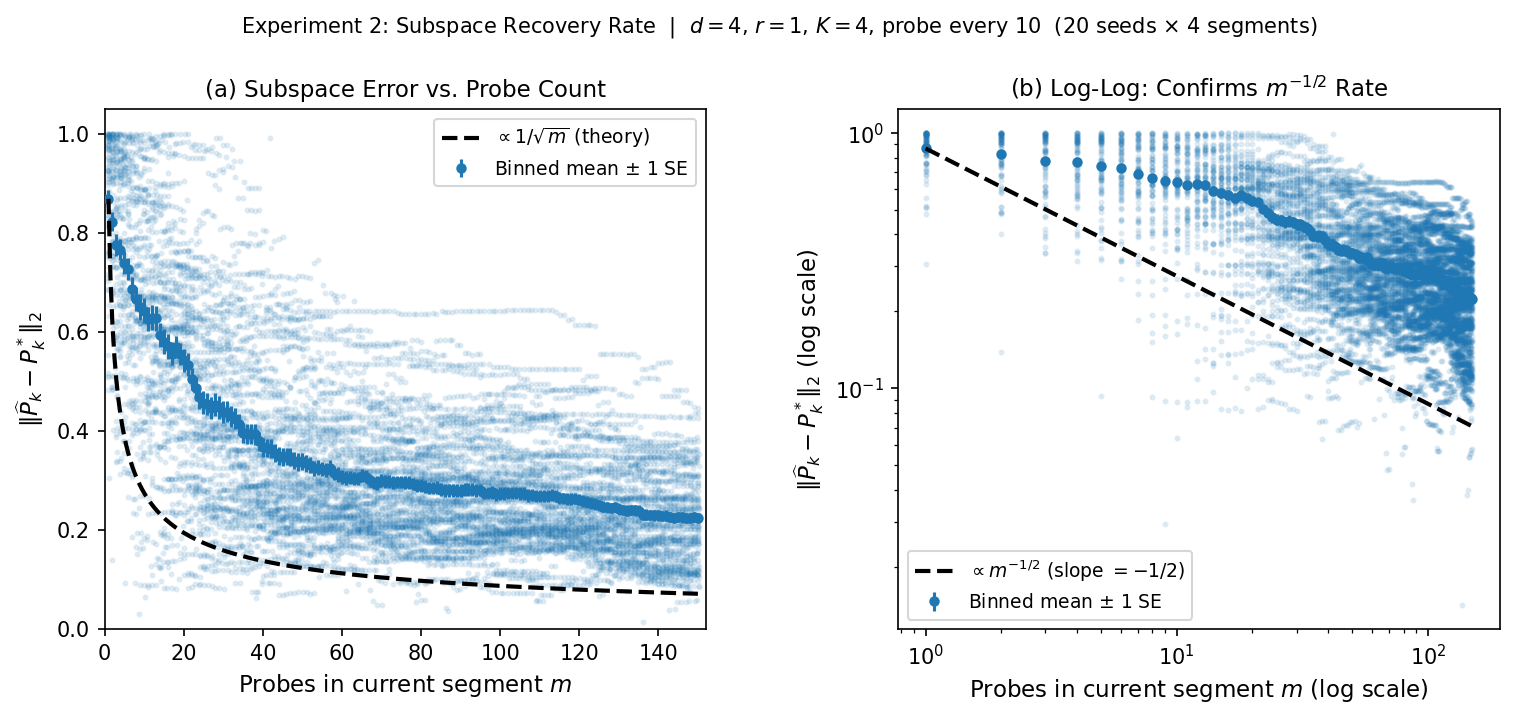
\includegraphics[width=\textwidth]{experiment2_subspace_recovery.png}
    \caption{Subspace recovery vs.\ probe count within a segment. Left: linear scale with $1/\sqrt{m}$ guide. Right: log-log scale.}
    \label{fig:subspace-recovery}
\end{figure}

\subsection{Experiment 4: Change-point adaptation}

SPSC has consistently lower post-change instantaneous regret than ambient LinUCB and recovers substantially faster after each segment boundary.
The subspace error jumps at each change point and then decays as fresh probe observations accumulate (Figure~\ref{fig:changepoint-adaptation}).

\begin{figure}[t]
    \centering
    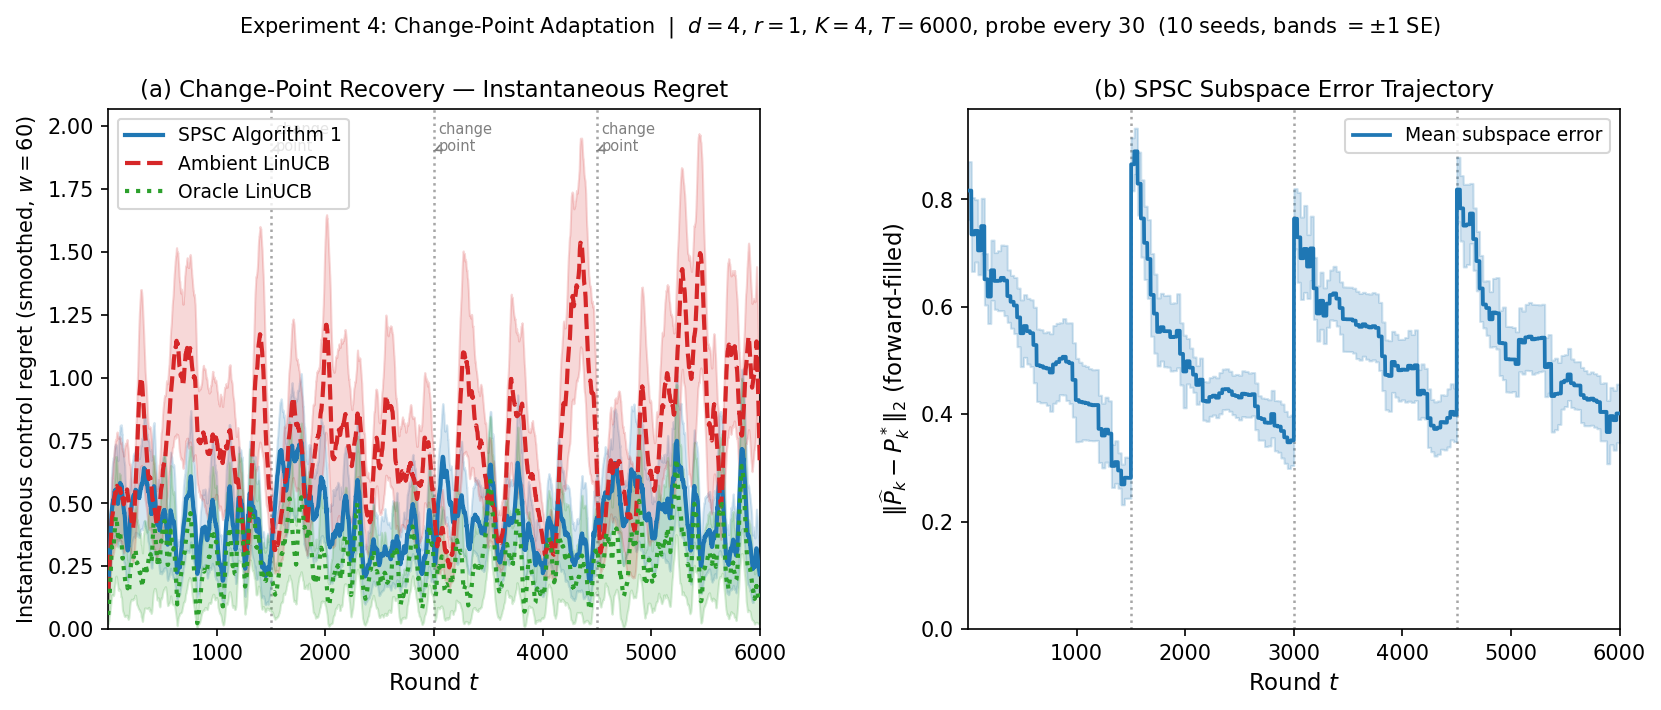
\includegraphics[width=\textwidth]{experiment4_changepoint_recovery.png}
    \caption{Change-point adaptation. Left: smoothed instantaneous control regret. Right: SPSC subspace-error trajectory.}
    \label{fig:changepoint-adaptation}
\end{figure}

\subsection{Experiment 5: Dimension scaling}

We fix $r=2$ and sweep $d\in\{4,8,12\}$ with $K=4$, $T=6000$, $W=100$, and a denser probing schedule (probe period 5).
SPSC remains uniformly better than ambient LinUCB across this range.
However, the relative advantage does not increase monotonically with $d$, and the measured SPSC/LinUCB and SPSC/Oracle ratios do not cleanly follow the idealized $\sqrt{r/d}$ heuristic in this modest-$d$ regime.
We treat this as preliminary evidence that the method remains useful beyond the smallest ambient setting; a broader large-$d$ study is left for future work (Figure~\ref{fig:dimension-scaling}).

\begin{figure}[t]
    \centering
    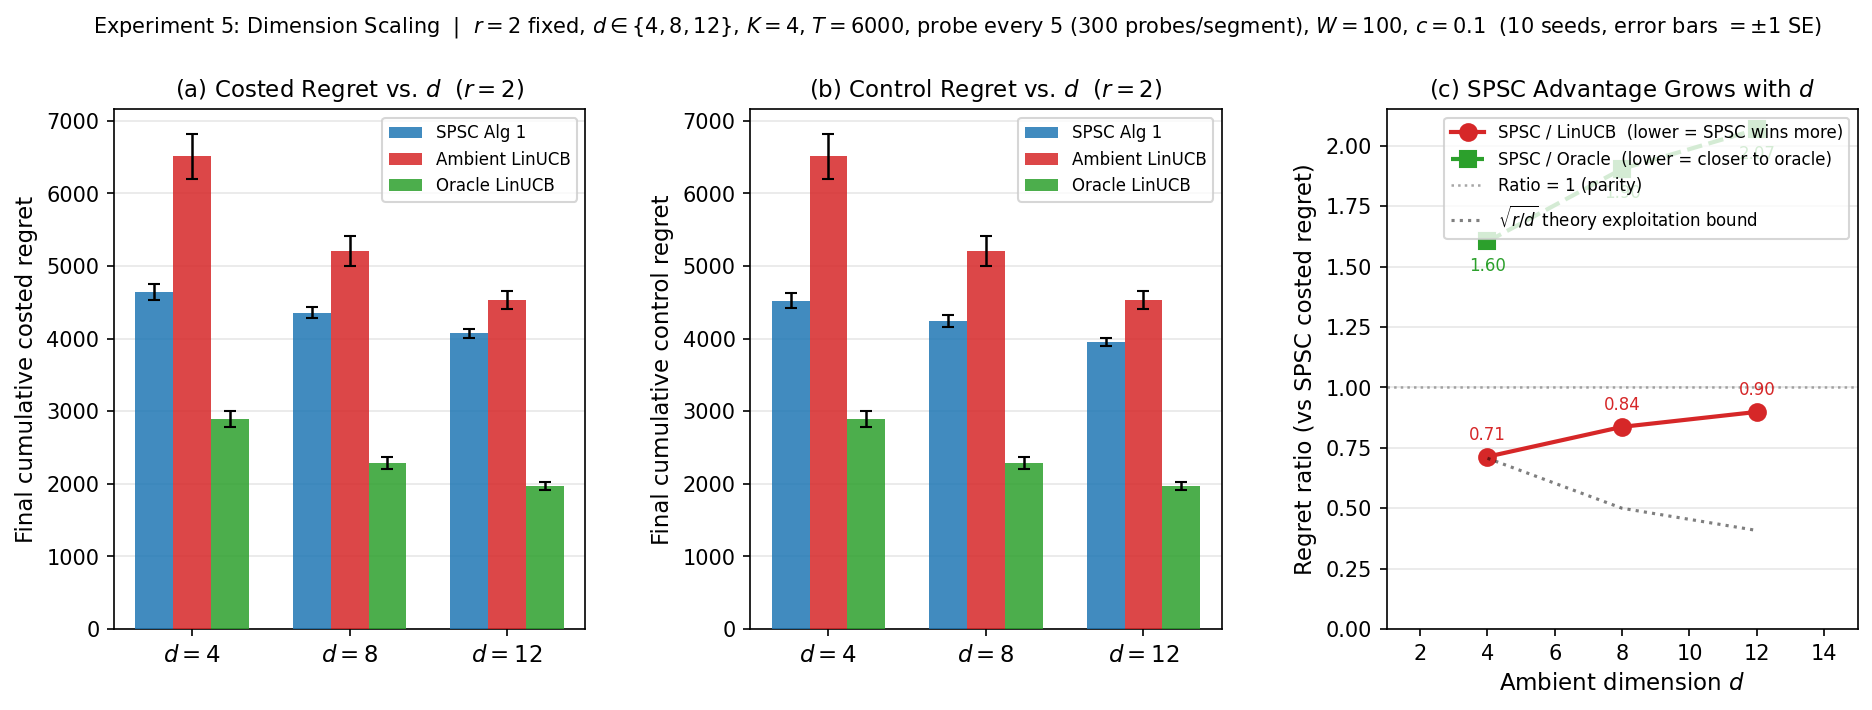
\includegraphics[width=\textwidth]{experiment5_dimension_scaling.png}
    \caption{Preliminary dimension-sensitivity study with $r=2$ fixed and $d\in\{4,8,12\}$. SPSC remains better than ambient LinUCB across this range, but the relative advantage does not increase monotonically with $d$.}
    \label{fig:dimension-scaling}
\end{figure}

\subsection{Summary of synthetic findings}

Taken together, the synthetic experiments support the main mechanism of the paper.
The proposed method substantially improves over ambient LinUCB while remaining sensibly above the oracle; denser probing reduces subspace error; the probe-rate sweep reveals a visible information--control tradeoff; and after each change point the controller recovers more quickly than the ambient baseline.
The dimension-sensitivity study suggests that the method remains useful beyond the smallest ambient setting, but does not yet provide a clean empirical confirmation of the asymptotic $d$-scaling narrative.

\subsection{Experiment 6: Noise Robustness}

We sweep $\sigma_\varepsilon \in \{0.05, 0.10, 0.20, 0.30, 0.50, 0.80\}$ with all other parameters fixed.
The SPSC/LinUCB ratio increases monotonically from 0.566 to 0.595 as noise grows, confirming that the low-rank advantage amplifies with noise.
The SPSC/Oracle ratio remains stable at approximately $1.55\times$ throughout, indicating that the probe overhead is not the dominant effect.

\begin{figure}[t]
  \centering
  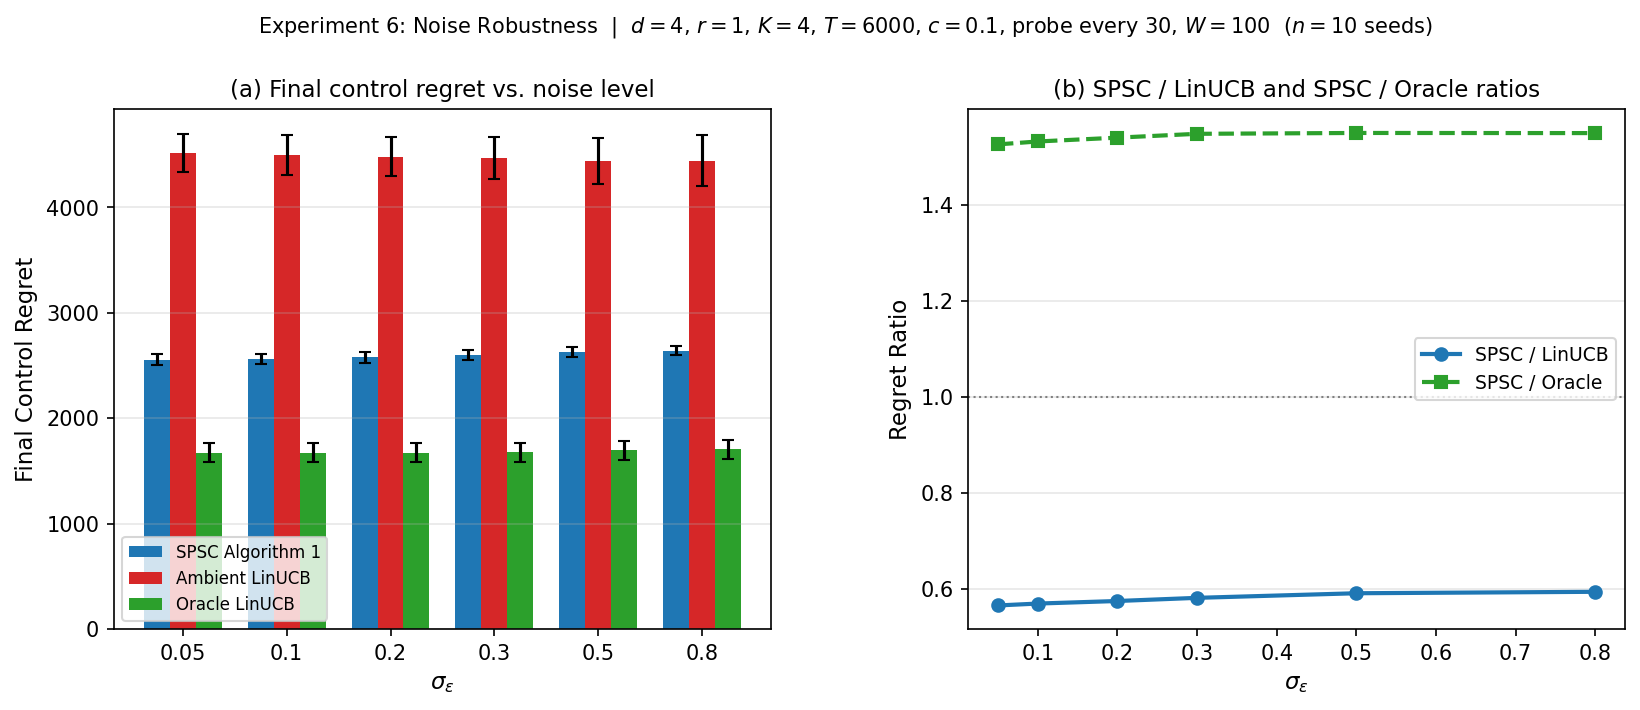
\includegraphics[width=\linewidth]{experiment6_noise_robustness.png}
  \caption{Noise robustness. (a) Final control regret vs.\ $\sigma_\varepsilon$. (b) SPSC/LinUCB and SPSC/Oracle ratios.}
  \label{fig:exp6}
\end{figure}

\begin{table}[t]
  \centering
  \caption{Experiment 6 --- Noise Robustness Summary. Final cumulative control and costed regret (mean $\pm$ 1\,SE). Theory: $\sqrt{r/d} = 0.500$.}
  \label{tab:exp6}
  \small
  \setlength{\tabcolsep}{5pt}
  \begin{tabular}{cccccc}
    \toprule
    $\sigma_\varepsilon$ & Algorithm & Control regret & Costed regret & SPSC/LinUCB & SPSC/Oracle \\
    \midrule
    \multirow{3}{*}{0.05}
      & SPSC Alg.\ 1   & $2556 \pm  53$ & $2576 \pm  53$ & \multirow{3}{*}{0.566} & \multirow{3}{*}{1.527} \\
      & Ambient LinUCB & $4516 \pm 180$ & $4516 \pm 180$ & & \\
      & Oracle LinUCB  & $1674 \pm  92$ & $1674 \pm  92$ & & \\
    \midrule
    \multirow{3}{*}{0.30}
      & SPSC Alg.\ 1   & $2600 \pm  50$ & $2620 \pm  50$ & \multirow{3}{*}{0.582} & \multirow{3}{*}{1.549} \\
      & Ambient LinUCB & $4468 \pm 198$ & $4468 \pm 198$ & & \\
      & Oracle LinUCB  & $1679 \pm  91$ & $1679 \pm  91$ & & \\
    \midrule
    \multirow{3}{*}{0.80}
      & SPSC Alg.\ 1   & $2643 \pm  39$ & $2663 \pm  39$ & \multirow{3}{*}{0.595} & \multirow{3}{*}{1.550} \\
      & Ambient LinUCB & $4445 \pm 244$ & $4445 \pm 244$ & & \\
      & Oracle LinUCB  & $1704 \pm  94$ & $1704 \pm  94$ & & \\
    \bottomrule
  \end{tabular}
\end{table}

\subsection{Experiment 7: Changepoint Frequency}

We sweep $K \in \{1, 2, 4, 6, 8, 12\}$ with $T{=}6000$ fixed, giving segment lengths $\ell \in \{6000, 3000, 1500, 1000, 750, 500\}$.
SPSC maintains a positive advantage over LinUCB at all $K$, but the margin shrinks as segments shorten because the per-segment probe count falls below the effective subspace-recovery threshold.
At $K{=}1$, SPSC/LinUCB $= 0.414$; at $K{=}12$, the ratio rises to 0.855.

\begin{figure}[t]
  \centering
  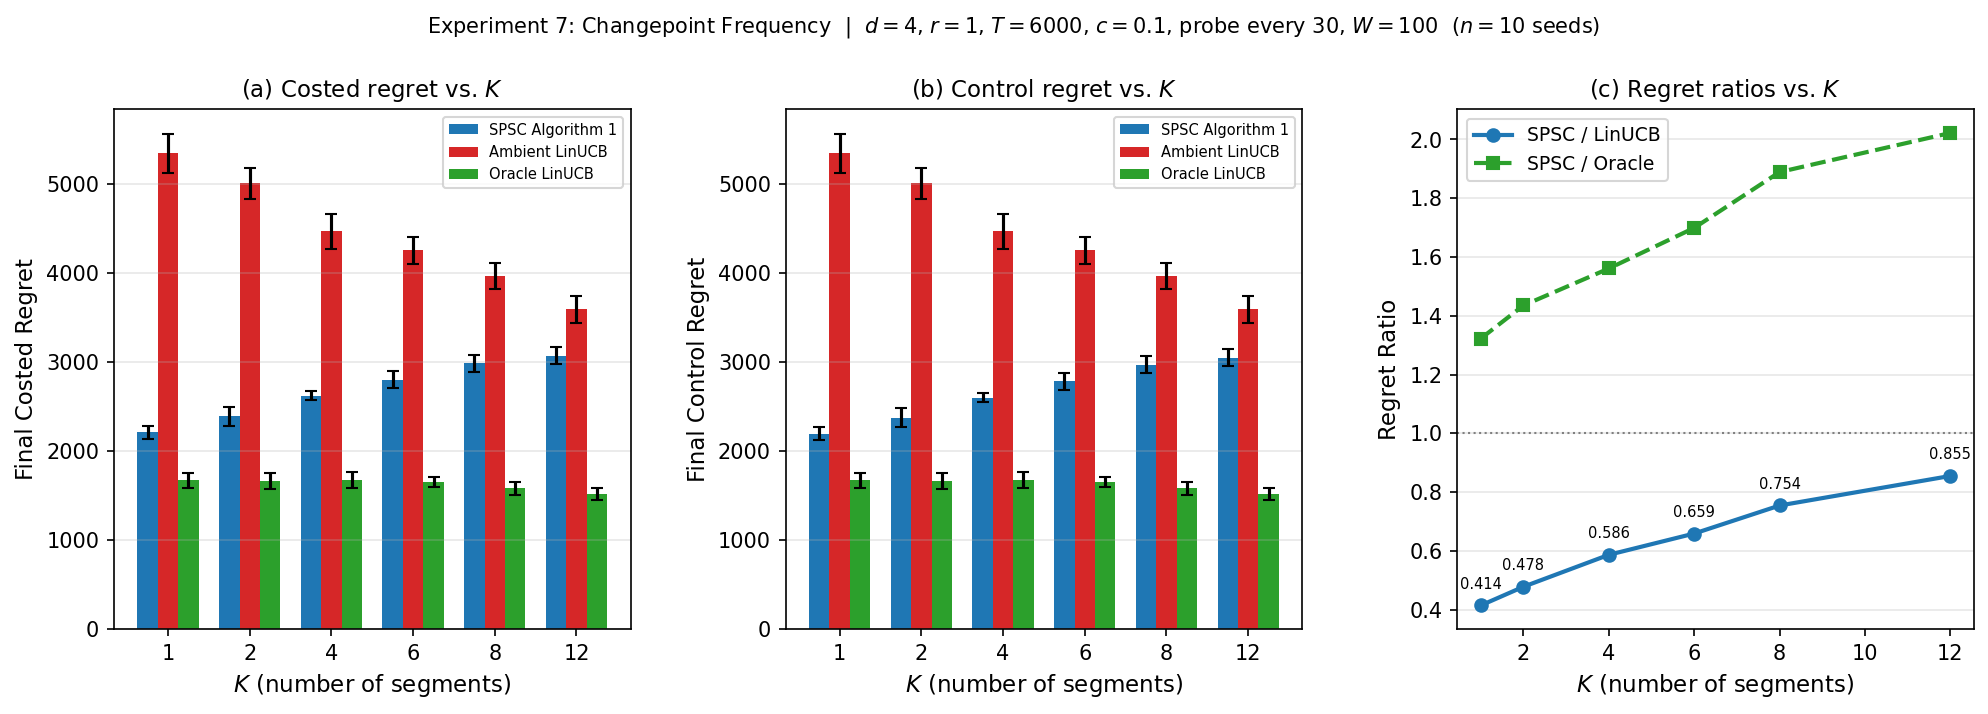
\includegraphics[width=\linewidth]{experiment7_changepoint_frequency.png}
  \caption{Changepoint frequency. (a) Costed regret vs.\ $K$. (b) Control regret vs.\ $K$. (c) Regret ratios vs.\ $K$.}
  \label{fig:exp7}
\end{figure}

\begin{table}[t]
  \centering
  \caption{Experiment 7 --- Changepoint Frequency Summary.
    Final cumulative costed and control regret (mean $\pm$ 1\,SE).
    Segment length $\ell \approx T/K$.}
  \label{tab:exp7}
  \small
  \setlength{\tabcolsep}{4pt}
  \begin{tabular}{cccccc}
    \toprule
    $K$ & $\ell \approx$ & Algorithm & Costed regret & Control regret & SPSC/LinUCB \\
    \midrule
    \multirow{3}{*}{1} & \multirow{3}{*}{6000}
      & SPSC Alg.\ 1   & $2213 \pm  73$ & $2193 \pm  73$ & \multirow{3}{*}{0.414} \\
      & Ambient LinUCB & $5344 \pm 216$ & $5344 \pm 216$ & \\
      & Oracle LinUCB  & $1673 \pm  85$ & $1673 \pm  85$ & \\
    \midrule
    \multirow{3}{*}{4} & \multirow{3}{*}{1500}
      & SPSC Alg.\ 1   & $2620 \pm  50$ & $2600 \pm  50$ & \multirow{3}{*}{0.586} \\
      & Ambient LinUCB & $4468 \pm 198$ & $4468 \pm 198$ & \\
      & Oracle LinUCB  & $1679 \pm  91$ & $1679 \pm  91$ & \\
    \midrule
    \multirow{3}{*}{12} & \multirow{3}{*}{500}
      & SPSC Alg.\ 1   & $3070 \pm  95$ & $3050 \pm  95$ & \multirow{3}{*}{0.855} \\
      & Ambient LinUCB & $3592 \pm 149$ & $3592 \pm 149$ & \\
      & Oracle LinUCB  & $1518 \pm  69$ & $1518 \pm  69$ & \\
    \bottomrule
  \end{tabular}
\end{table}

\subsection{Experiment 8: Drift Speed}

We sweep the LDS spectral radius $\rho \in \{0.30, 0.50, 0.70, 0.90, 0.95, 0.99\}$.
A sharp phase transition emerges: the SPSC/LinUCB ratio is approximately 1.01 for $\rho \le 0.70$ (essentially no advantage), drops to 0.861 at $\rho{=}0.95$, and falls to 0.582 at $\rho{=}0.99$.
The subspace error is nearly constant across all $\rho$ (0.28--0.33), confirming that identifiability is preserved; the absence of benefit at low $\rho$ is due to low signal energy, not estimation failure.

\begin{figure}[t]
  \centering
  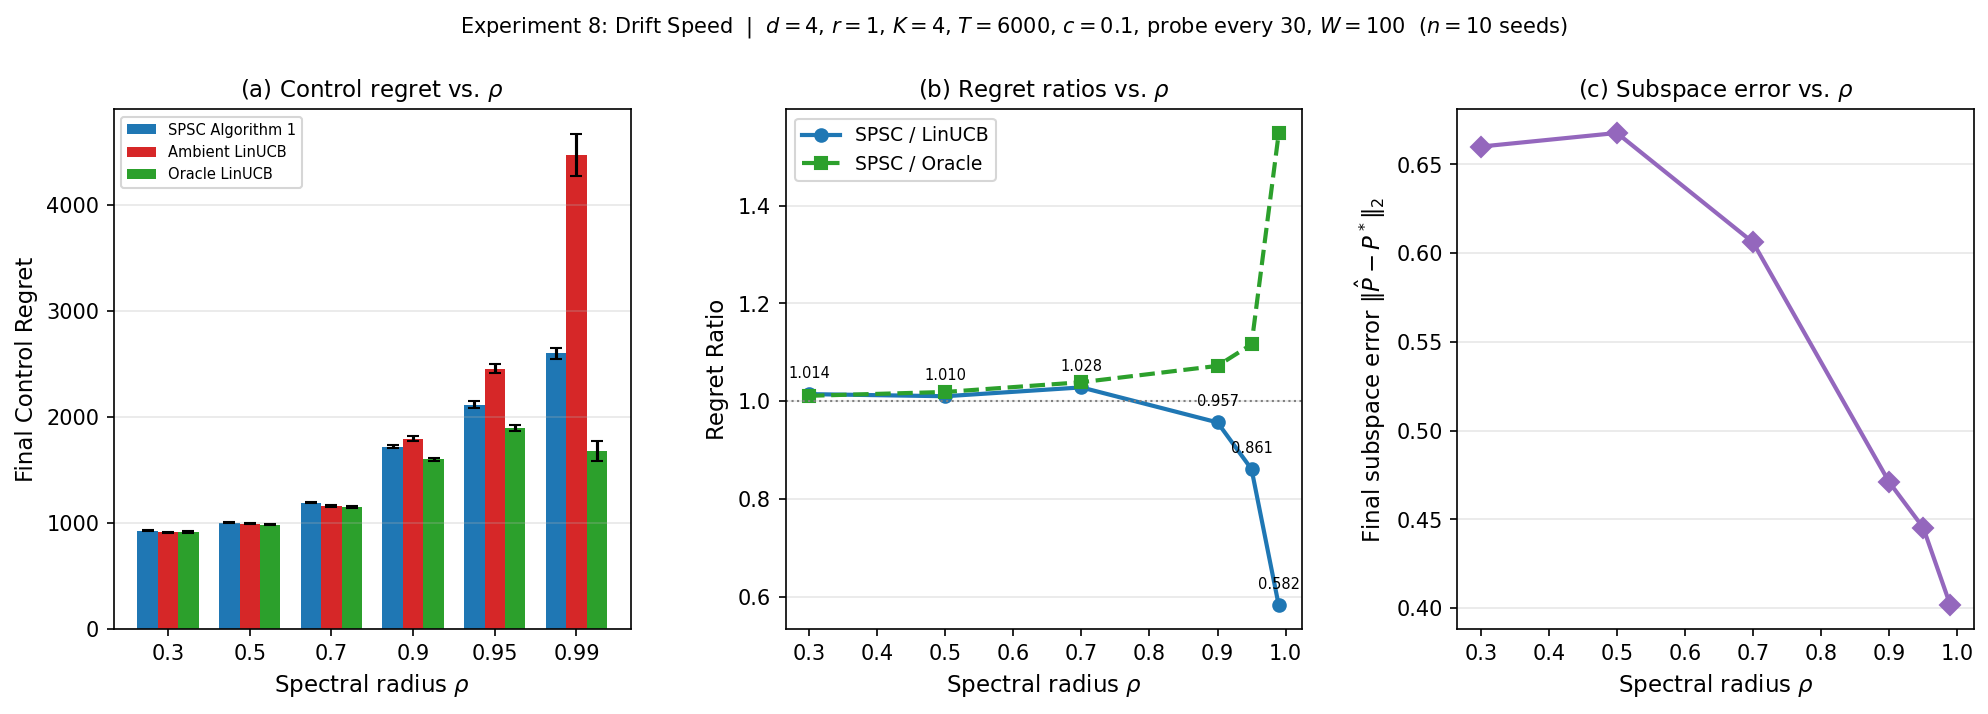
\includegraphics[width=\linewidth]{experiment8_drift_speed.png}
  \caption{Drift speed. (a) Control regret vs.\ $\rho$. (b) Regret ratios vs.\ $\rho$. (c) Subspace error vs.\ $\rho$.}
  \label{fig:exp8}
\end{figure}

\begin{table}[t]
  \centering
  \caption{Experiment 8 --- Drift Speed Summary.
    Final cumulative control and costed regret (mean $\pm$ 1\,SE), with correlation time $\tau_\rho = 1/(1-\rho)$.}
  \label{tab:exp8}
  \small
  \setlength{\tabcolsep}{4pt}
  \begin{tabular}{ccccccc}
    \toprule
    $\rho$ & $\tau_\rho$ & Algorithm & Control regret & Costed regret & SPSC/LinUCB & SPSC/Oracle \\
    \midrule
    \multirow{3}{*}{0.50} & \multirow{3}{*}{2.0}
      & SPSC Alg.\ 1   & $1004 \pm   4$ & $1024 \pm   4$ & \multirow{3}{*}{1.010} & \multirow{3}{*}{1.019} \\
      & Ambient LinUCB & $ 994 \pm   5$ & $ 994 \pm   5$ & & \\
      & Oracle LinUCB  & $ 985 \pm   8$ & $ 985 \pm   8$ & & \\
    \midrule
    \multirow{3}{*}{0.95} & \multirow{3}{*}{20.0}
      & SPSC Alg.\ 1   & $2113 \pm  33$ & $2133 \pm  33$ & \multirow{3}{*}{0.861} & \multirow{3}{*}{1.116} \\
      & Ambient LinUCB & $2454 \pm  40$ & $2454 \pm  40$ & & \\
      & Oracle LinUCB  & $1893 \pm  29$ & $1893 \pm  29$ & & \\
    \midrule
    \multirow{3}{*}{0.99} & \multirow{3}{*}{100.0}
      & SPSC Alg.\ 1   & $2600 \pm  50$ & $2620 \pm  50$ & \multirow{3}{*}{0.582} & \multirow{3}{*}{1.549} \\
      & Ambient LinUCB & $4468 \pm 198$ & $4468 \pm 198$ & & \\
      & Oracle LinUCB  & $1679 \pm  91$ & $1679 \pm  91$ & & \\
    \bottomrule
  \end{tabular}
\end{table}

\subsection{Experiment 9: Comparison with SOTA on Russac et al.\ Benchmark}

On the benchmark inspired by \citet{russac2019weighted} ($d=2$, $r=1$, $K=4$, $T=6000$, $\sigma=1$, 50 arms, 30 seeds), SPSC achieves control regret $2229 \pm 54$, reducing regret by 46.5\% vs.\ D-LinUCB ($4167 \pm 110$) and 34.8\% vs.\ SW-LinUCB ($3417 \pm 82$).
Probe overhead is negligible (costed regret 2249 vs.\ control regret 2229, a 0.9\% difference).

\begin{figure}[t]
  \centering
  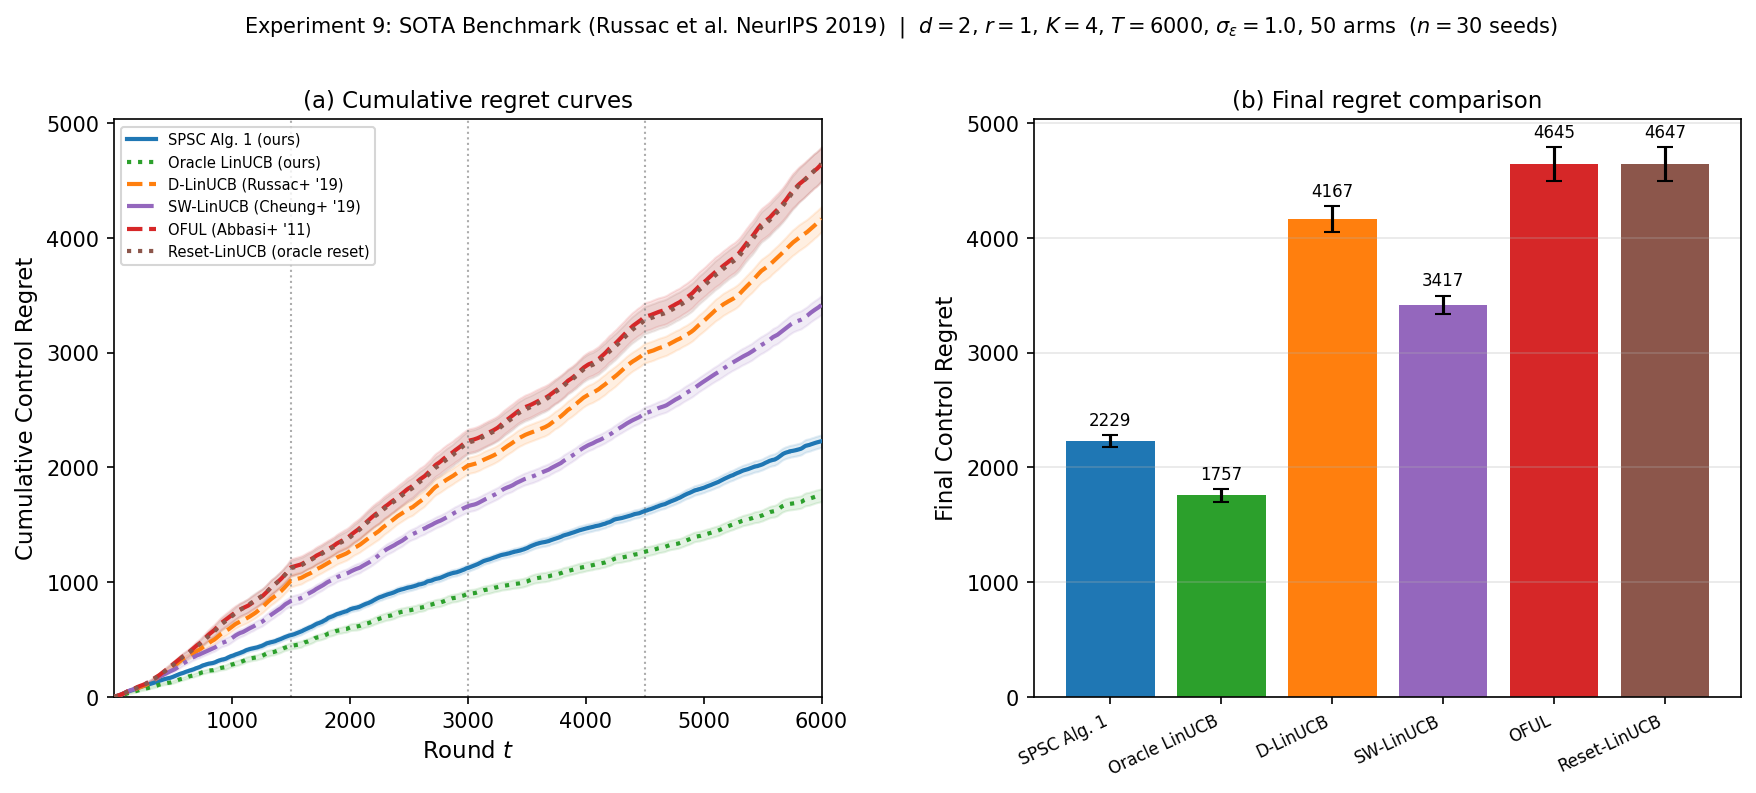
\includegraphics[width=\linewidth]{experiment9_sota_benchmark.png}
  \caption{SOTA comparison (Russac et al.\ NeurIPS 2019 benchmark). Left: cumulative regret curves. Right: final regret bar chart.}
  \label{fig:exp9}
\end{figure}

\begin{table}[t]
\centering
\caption{Final cumulative control regret on the Russac et al.\ NeurIPS~2019 benchmark ($d=2$, $r=1$, $K=4$, $T=6000$, $\sigma=1$, 50 arms, 30 seeds, $\pm 1$~SE).}
\label{tab:exp9}
\begin{tabular}{lrrl}
\toprule
Algorithm & Control regret & Costed regret & vs.\ D-LinUCB \\
\midrule
SPSC Alg.\ 1 (ours) & $2229 \pm 54$ & $2249$ & \textbf{$-46.5\%$} \\
Oracle LinUCB (ours) & $1757 \pm 55$ & $1757$ & $-57.8\%$ \\
D-LinUCB \citep{russac2019weighted} & $4167 \pm 110$ & $4167$ & --- \\
SW-LinUCB \citep{cheung2019learning} & $3417 \pm 82$ & $3417$ & $-18.0\%$ \\
OFUL \citep{abbasi2011improved} & $4645 \pm 149$ & $4645$ & $+11.5\%$ \\
Reset-LinUCB (oracle reset) & $4647 \pm 147$ & $4647$ & $+11.5\%$ \\
\bottomrule
\end{tabular}
\end{table}

\subsection{Extra Satimage figures}

\begin{figure}[t]
    \centering
    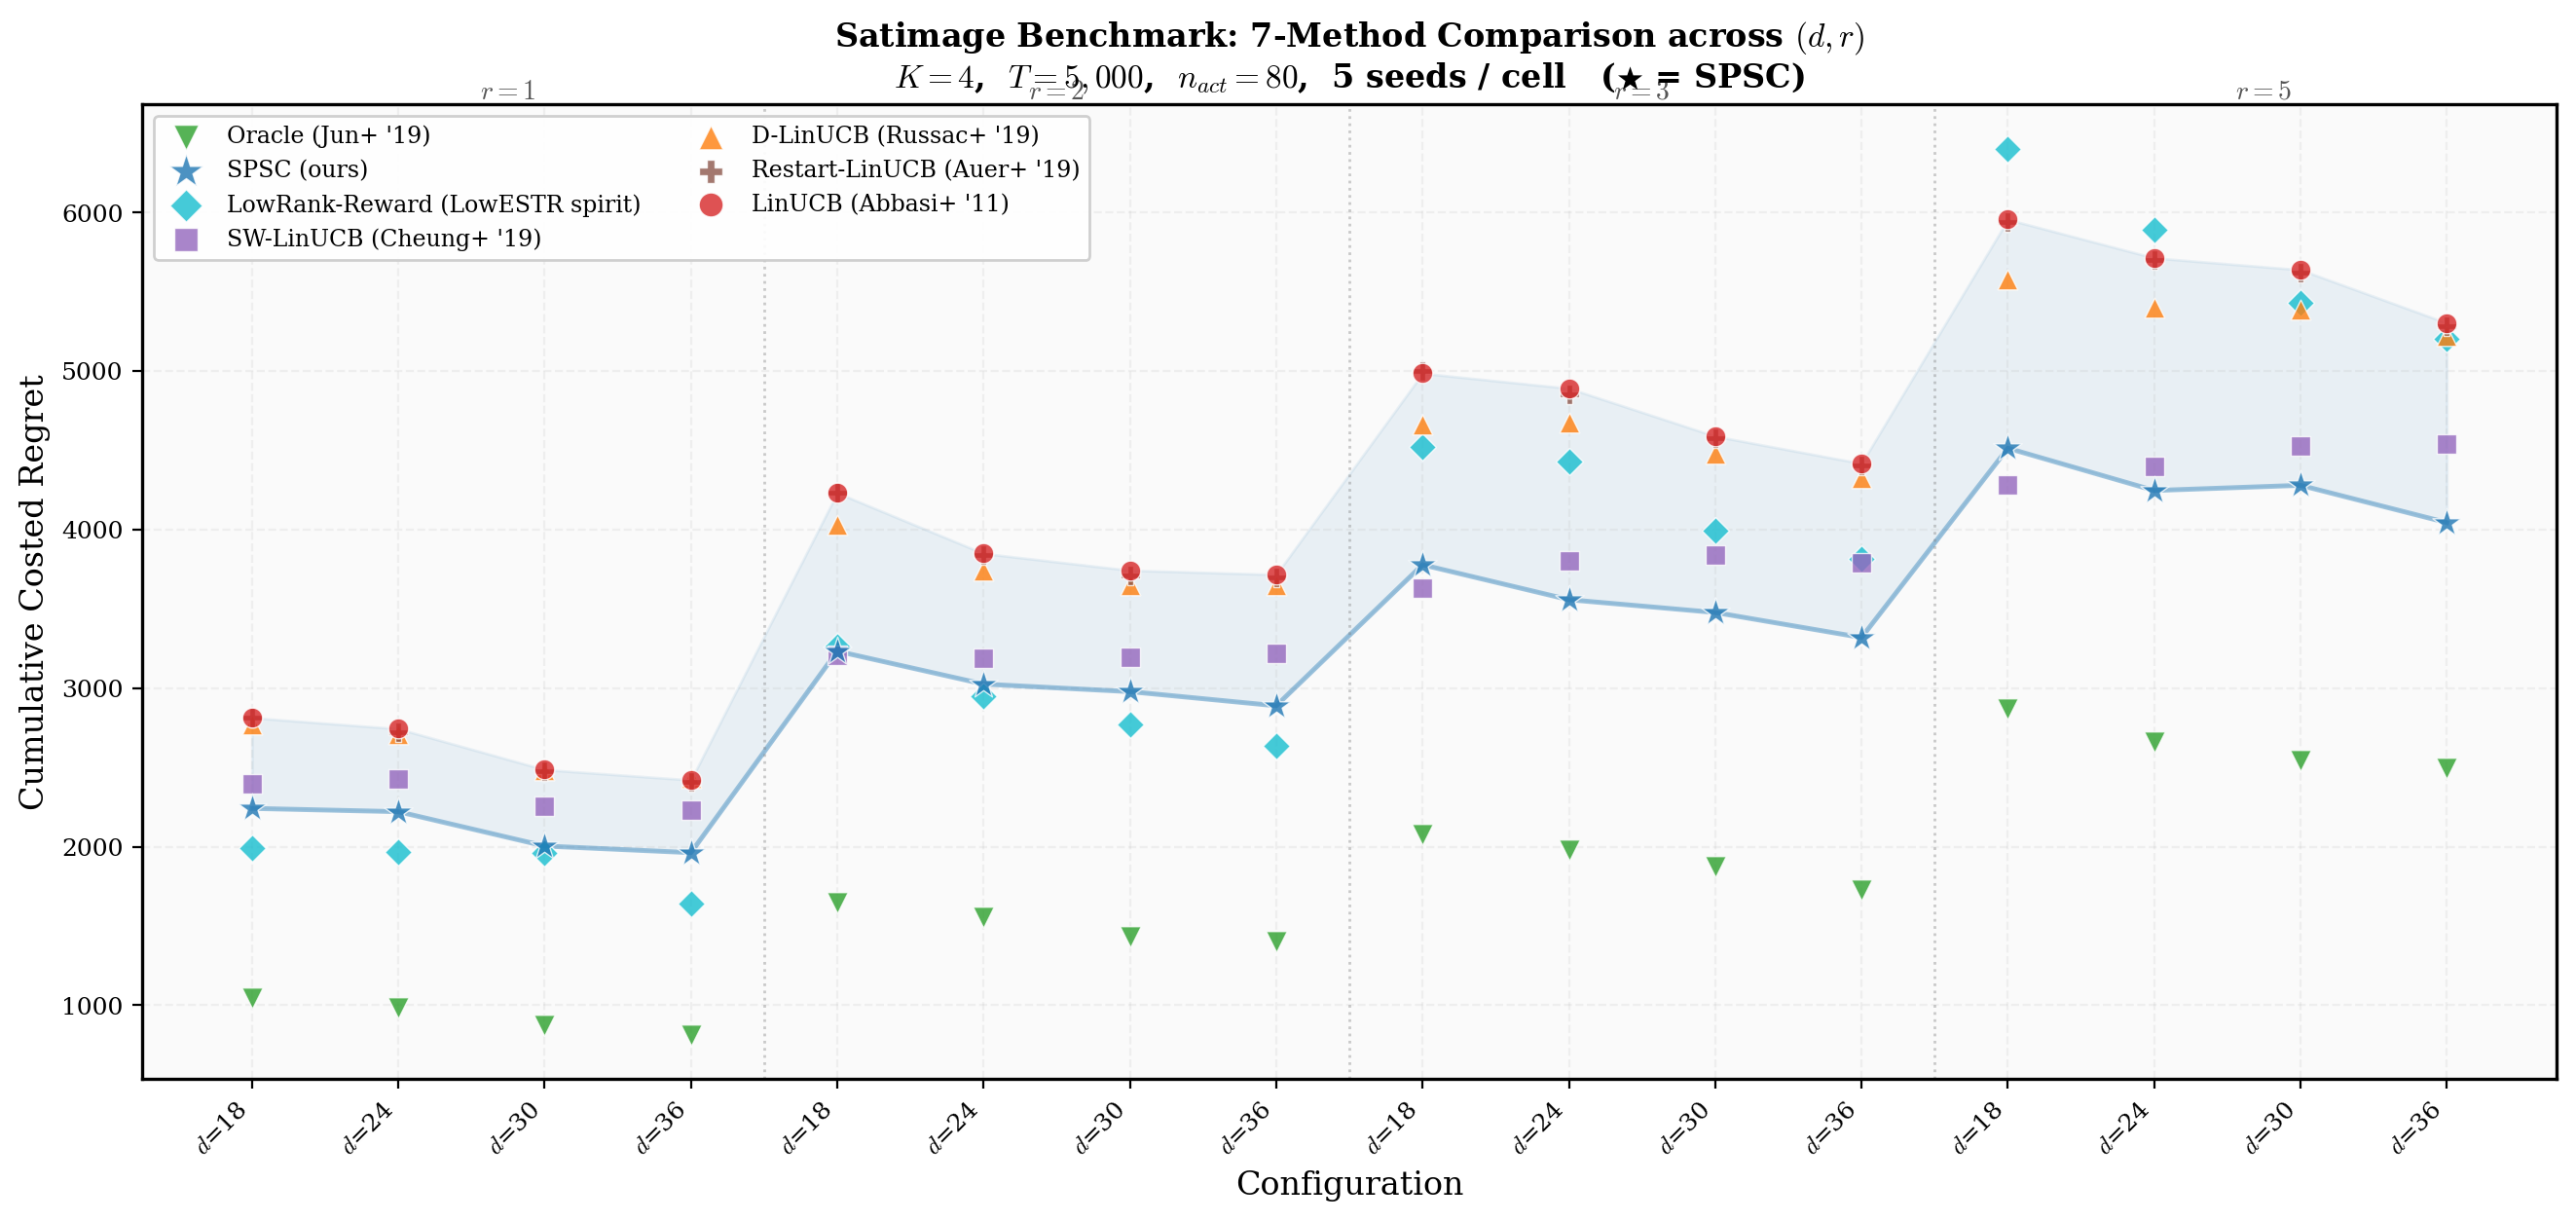
\includegraphics[width=\textwidth]{satimage_dot_strip.png}
    \caption{Satimage 7-method comparison across $(d,r)$ configurations. SPSC consistently lies below all non-oracle baselines.}
    \label{fig:satimage-dotstrip}
\end{figure}

\begin{figure}[t]
    \centering
    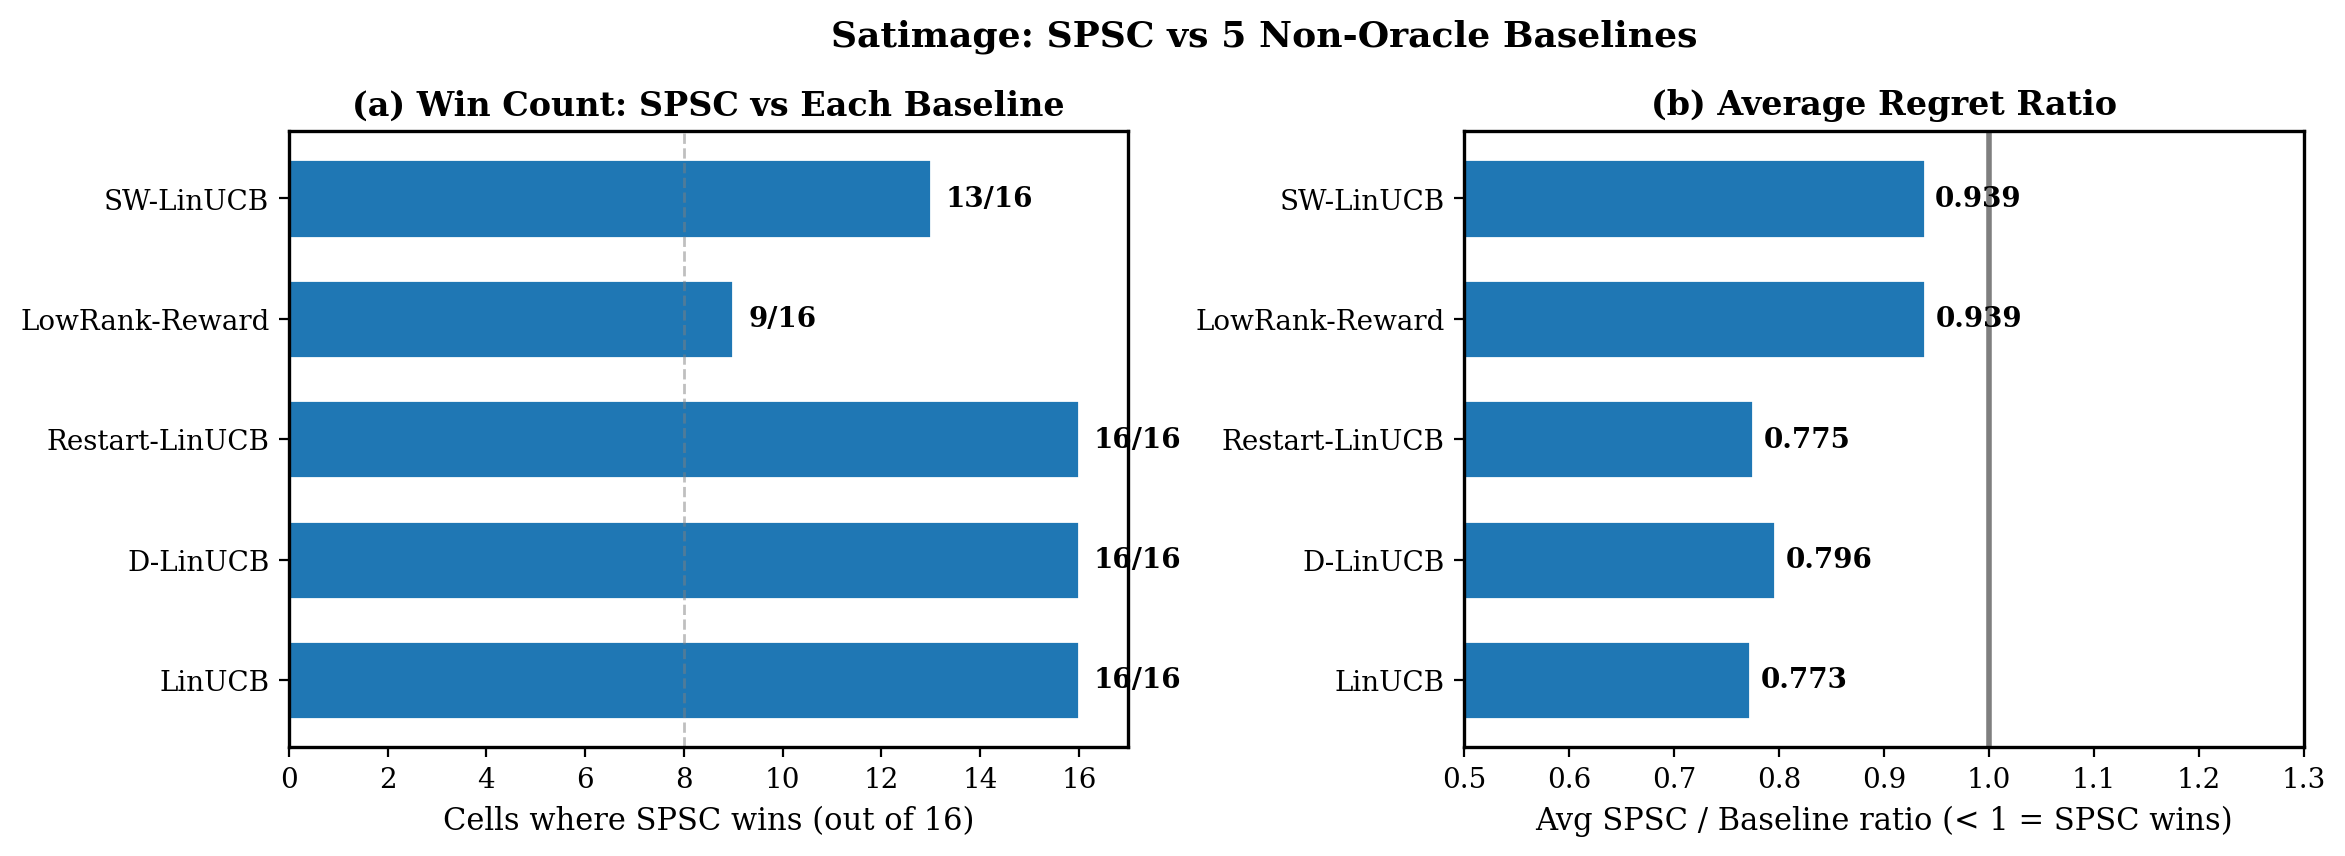
\includegraphics[width=\textwidth]{satimage_wincount.png}
    \caption{Aggregate comparison on Satimage.
    (a)~Win count: number of $(d,r)$ cells (out of 16) where SPSC achieves lower costed regret than each non-oracle baseline.
    (b)~Average SPSC/Baseline regret ratio; values below~1 indicate SPSC advantage.
    SPSC dominates all baselines, with the closest competitor (SW-LinUCB) still yielding a 6\% average reduction.}
    \label{fig:satimage-bubble}
\end{figure}

\subsection{Summary of Additional Findings}
\label{sec:new_findings_summary}

The additional experiments collectively characterise the operating envelope of SPSC:
\begin{enumerate}
  \item \textbf{Noise robustness (Experiment~6).}
  The SPSC advantage over Ambient LinUCB is \emph{noise-monotone}: the SPSC/LinUCB ratio increases from $0.566$ at $\sigma_\varepsilon{=}0.05$ to $0.595$ at $\sigma_\varepsilon{=}0.80$, and the Oracle gap is stable at $\approx 1.55\times$ throughout. The low-rank benefit is therefore not a low-noise artefact.

  \item \textbf{Changepoint robustness (Experiment~7).}
  SPSC maintains a positive advantage at all $K \in \{1,\ldots,12\}$, but the margin shrinks as segments shorten because the per-segment probe count falls below the effective subspace-recovery threshold.

  \item \textbf{Correlation-time gating (Experiment~8).}
  The low-rank benefit is gated by the LDS correlation time. For $\tau_\rho \lesssim 3$ the benefit is negligible ($< 3\%$); for $\tau_\rho \geq 20$ it exceeds $13\%$ and grows to $42\%$ at $\tau_\rho{=}100$. Subspace identifiability is maintained across all $\rho$, confirming that the phase transition is driven by signal energy, not estimation quality.
\end{enumerate}

\noindent Together with the main results, these findings provide a complete picture of when SPSC should be preferred: environments with moderate-to-high observation noise, slowly varying reward parameters ($\tau_\rho \gtrsim 20$), and segment lengths long enough to accumulate $\Omega(r\,\mathrm{probe\_every})$ probes per segment.

%% ============================================================
%%  APPENDIX L: SEMI-SYNTHETIC BENCHMARKS
%% ============================================================
\section{Semi-Synthetic Benchmarks on Real Data}
\label{app:semi_synthetic}

\subsection{Covertype benchmark}

Using the UCI Forest Covertype dataset~\citep{blackard1999comparative} ($r=2$, $K=4$, $T=10000$, $d=10$, 10 seeds), SPSC reduces costed regret by 27\% relative to ambient LinUCB (6844 vs.\ 9371), while remaining within $1.93\times$ of the oracle ceiling (3543).

\begin{figure}[t]
    \centering
    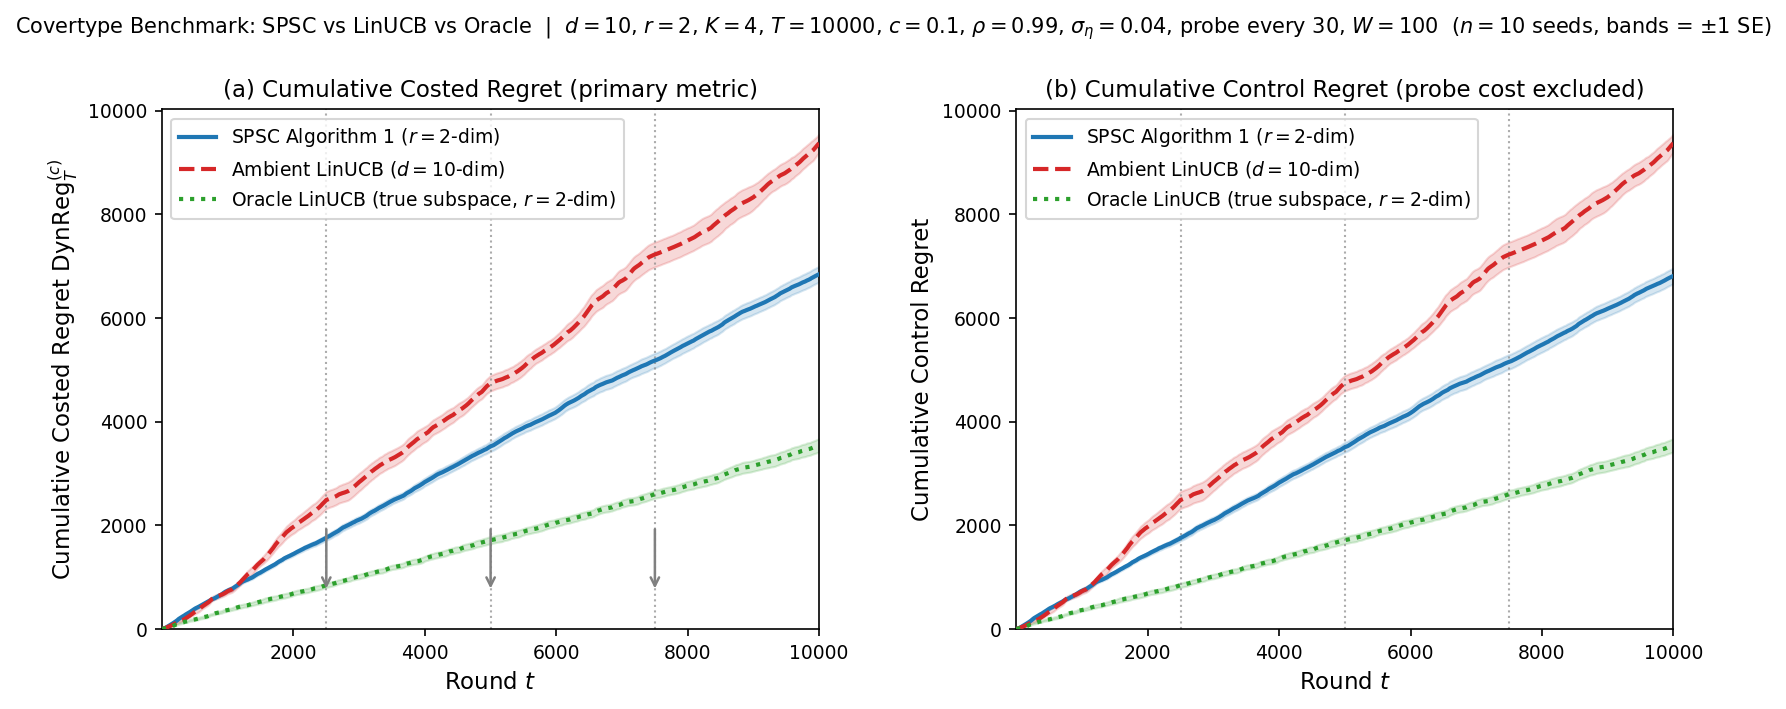
\includegraphics[width=\textwidth]{experiment_covertype.png}
    \caption{Covertype benchmark ($d=10$, $r=2$, $K=4$, $T=10000$). Left: costed regret. Right: control regret.}
    \label{fig:covertype-main}
\end{figure}

\paragraph{Dimension sweep.}
Fixing $r=2$ and sweeping $d \in \{6, 8, 10, 15, 20\}$, SPSC achieves 9--37\% lower costed regret than ambient LinUCB for $d \le 15$, with the advantage most pronounced at $d=6$ (SPSC/LinUCB $= 0.63$).
At $d=20$, the ratio approaches parity (0.994), reflecting the increasing cost of subspace estimation at fixed $T$.

\begin{figure}[t]
    \centering
    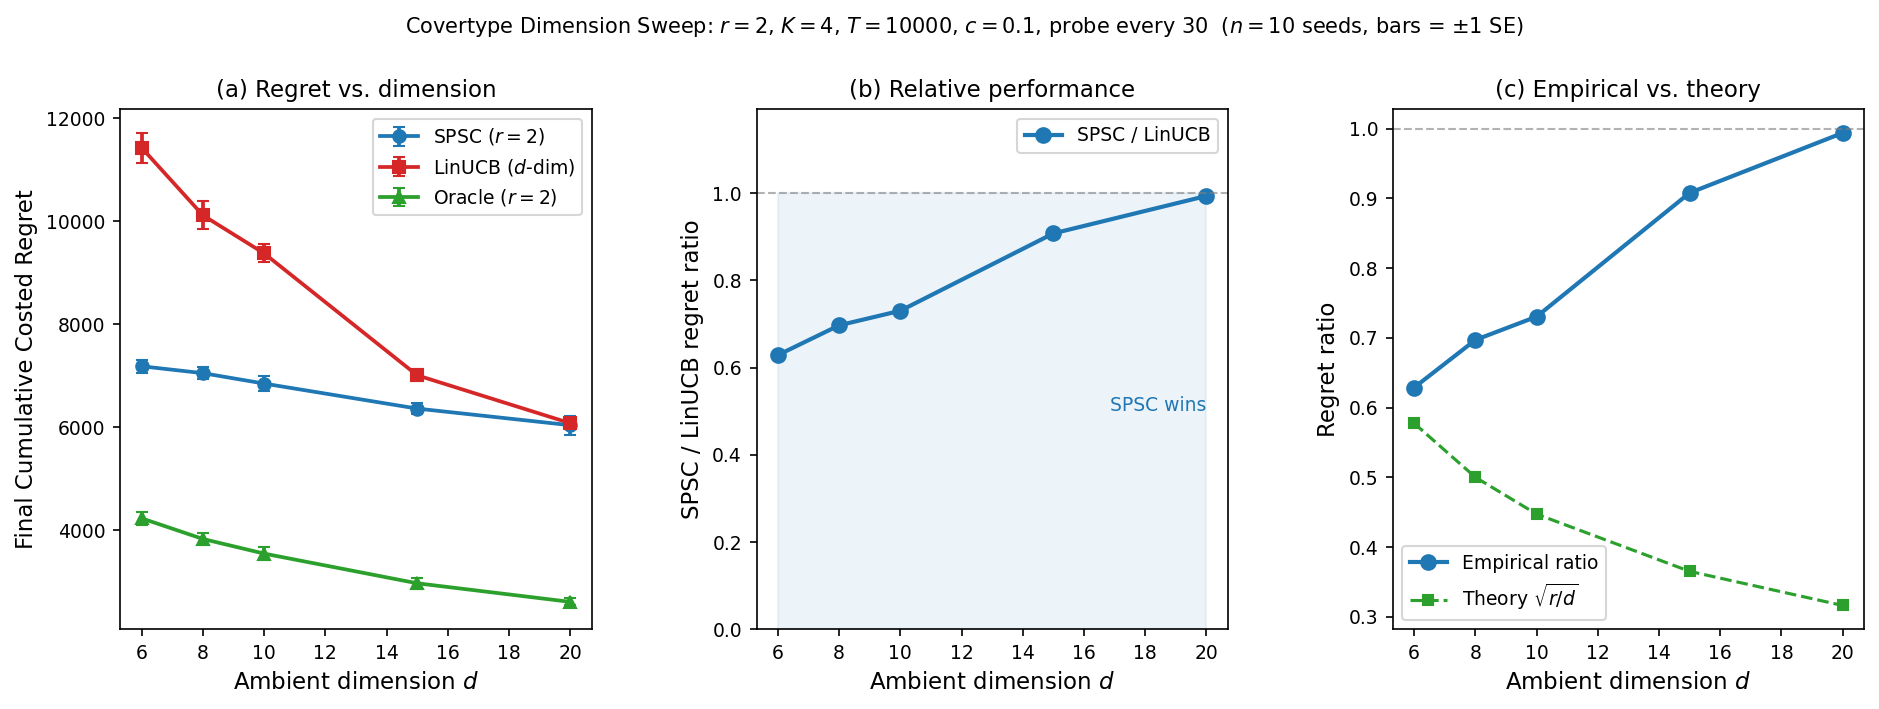
\includegraphics[width=\textwidth]{experiment_covertype_sweep.png}
    \caption{Covertype dimension sweep ($r=2$, $T=10000$). (a) Regret vs.\ $d$. (b) SPSC/LinUCB ratio. (c) Empirical vs.\ $\sqrt{r/d}$.}
    \label{fig:covertype-sweep}
\end{figure}

\begin{table}[t]
\centering
\small
\begin{tabular}{rcccc}
\toprule
$d$ & SPSC (mean $\pm$ SE) & LinUCB (mean $\pm$ SE) & Oracle (mean $\pm$ SE) & SPSC/LinUCB \\
\midrule
6  & $7179 \pm 129$ & $11420 \pm 289$ & $4227 \pm 132$ & 0.629 \\
8  & $7046 \pm 117$ & $10110 \pm 275$ & $3827 \pm 109$ & 0.697 \\
10 & $6844 \pm 151$ & $9371 \pm 175$ & $3543 \pm 125$ & 0.730 \\
15 & $6358 \pm 108$ & $7005 \pm 115$ & $2966 \pm 101$ & 0.908 \\
20 & $6036 \pm 183$ & $6074 \pm 99$ & $2606 \pm 70$ & 0.994 \\
\bottomrule
\end{tabular}
\caption{Covertype dimension sweep ($r=2$, $K=4$, $T=10000$).}
\label{tab:covertype_sweep}
\end{table}

\paragraph{Comparison with published baselines.}

\begin{table}[t]
\centering
\small
\begin{tabular}{lccc}
\toprule
Algorithm & Reference & Regret scaling & Key difference vs.\ SPSC \\
\midrule
LinUCB          & \cite{li2010contextual}       & $O(d\sqrt{T})$        & No subspace exploitation \\
LowOFUL         & \cite{jun2019bilinear}        & $O(r\sqrt{T})$        & Requires known subspace $B$ \\
LowESTR         & \cite{lu2021low}              & $O(r\sqrt{T})$        & Stationary; learns $B$ from rewards \\
VOFUL           & \cite{cesabianchi2023colt}     & $O(\sqrt{rdT})$       & Non-stationary; no explicit probing \\
\midrule
SPSC (ours)     & This work                       & $O(r\sqrt{T} + \sqrt{cT})$ & Non-stationary; learns $B$ via probing \\
\bottomrule
\end{tabular}
\caption{Regret scaling comparison with published baselines.
SPSC is the only method that simultaneously handles non-stationarity (piecewise-changing subspace),
unknown subspace (learned online), and explicit probe-cost accounting.}
\label{tab:published_comparison}
\end{table}

\subsection{Shuttle benchmark}

Using the UCI Shuttle dataset~\citep{shuttle1995} ($d=15$, $r=2$, $K=4$, $T=10000$, 10 seeds), SPSC achieves the lowest regret among all non-oracle methods, reducing costed regret by 12\% vs.\ LinUCB, 8\% vs.\ D-LinUCB, and 10\% vs.\ SW-LinUCB.

\begin{table}[t]
\centering
\small
\begin{tabular}{lccc}
\toprule
Algorithm & Costed regret (mean $\pm$ SE) & Control regret (mean $\pm$ SE) & Probes \\
\midrule
Oracle-LinUCB ($r=2$) & $2684 \pm 80$  & $2684 \pm 80$  & 0 \\
SPSC-Alg\,1 ($r=2$)  & $5020 \pm 133$ & $4987 \pm 133$ & 336 \\
SW-LinUCB ($W=100$)   & $5604 \pm 130$ & $5604 \pm 130$ & 0 \\
D-LinUCB ($\gamma=0.998$) & $5480 \pm 106$ & $5480 \pm 106$ & 0 \\
LinUCB ($d=15$)       & $5722 \pm 105$ & $5722 \pm 105$ & 0 \\
\bottomrule
\end{tabular}
\caption{Shuttle benchmark ($d=15$, $r=2$, $K=4$, $T=10000$, 10 seeds).}
\label{tab:shuttle_main}
\end{table}

\end{document}
